% Русский перевод статьи Casimir_honeycomb_drive.tex (опубликована: DOI 10.26565/2222-5617-2024-41-04).
% Рабочий вариант для осмысления; оригинал — английский.
\documentclass[twoside, 10pt]{article}

\usepackage[T1, T2A]{fontenc}   % Standard package for selecting font encodings
\usepackage[utf8]{inputenc} % Accept different input encodings
\usepackage[english, ukrainian, russian]{babel}

\usepackage{mathptmx}

\usepackage{indentfirst}    % Indent first paragraph after section header

\usepackage{sectsty}        % Control sectional headers
%\allsectionsfont{\mdseries\scshape\textbf}

\sectionfont{\normalfont\Large\textbf}
\subsectionfont{\normalfont\large\textbf}

\usepackage{multicol}       % Intermix single and multiple columns
\usepackage{orcidlink}      % Insert hyperlinked ORCiD logo
\usepackage{fancyhdr}       % Extensive control of page headers and footers

\usepackage{filecontents}
\usepackage{hyperref, doi}
\usepackage[numbers]{natbib}

\bibliographystyle{myunsrtnat}

\def\myfirstpage{28}
\def\mylastpage{41}
\def\mypages{\myfirstpage-\mylastpage}

\def\myfilename{Casimir_honeycomb_drive_ru}
\def\myname{А. Дроздов}
\def\mynameukr{А. Дроздов}
\def\mytitle{Сотовый двигатель Казимира: о силе, действующей на идеально проводящие соты на пластине}
\def\mytitleukr{Стільниковий рушій Казимира: про силу, що діє на соти на пластині, які ідеально проводять}
\def\myissn{2222-5617}
\def\mydoi{10.26565/2222-5617-2024-41-04}
\def\myemail{alexey.drozdov.07@gmail.com}
\def\ukrvisnyk{Вісник Харківського національного університету імені В.~Н.~Каразіна, серія «Фізика», вип. 41, \mypages~(2024)}
\def\envisnyk{Вестник Харьковского национального университета имени В.~Н.~Каразина, серия «Физика», вып. 41, \mypages~(2024)}
\def\myworkplace{Харьковский национальный университет имени В.~Н.~Каразина, пл. Свободы, 4, 61022 Харьков, Украина}
\def\myworkplaceukr{Харківський національний університет імені В.~Н.~Каразіна, майдан Свободи, 4, 61022 Харків, Україна}
\def\myorcidlink{0009-0004-1386-4534}

\def\myreceived{Поступила в редакцию 18 октября 2023 г. Рецензирована 16 ноября 2023 г.}
\def\myaccepted{Принята к печати 18 июня 2024 г.}
\def\myreceivedukr{Надійшла до редакції 18 жовтня 2023 р. Переглянуто 16 листопада 2023.}
\def\myacceptedukr{Прийнято до друку 18 червня 2024 р.}


\def\licenseref{http://creativecommons.org/licenses/by/4.0/}

\def\myvspacebeforesubsection{-2.0mm}
\def\myvspaceaftersubsection{-2.5mm}

\def\collontitulasfontcode{lmss}

\newcommand{\MyTitle}{\expandafter\MakeUppercase\expandafter{\mytitle}}
\newcommand{\MyTitleUkr}{\expandafter\MakeUppercase\expandafter{\mytitleukr}}

\fancypagestyle{firstpagestyle}{
% Definition of the header
\renewcommand{\headrulewidth}{0.6pt} % top horizontal rule
% Arial 9.5
\fancyhead[C]{\ukrvisnyk \\ \envisnyk}
\renewcommand{\footrulewidth}{0.6pt} % bottom horizontal rule
\fancyfoot[L]{${}^{\copyright}$ \myname}
\fancyfoot[R]{~ \\ \fontencoding{T1}\fontfamily{\collontitulasfontcode}{\selectfont \textit{Open Access. This article is licensed under a Creative Commons Attribution 4.0}} \\
\href{\licenseref}{\fontencoding{T1}\fontfamily{\collontitulasfontcode}{\selectfont \textit{\licenseref}}}}
}

    % Basic figure setup, for now with no caption control since it's done
    % automatically by Pandoc (which extracts ![](path) syntax from Markdown).
    \usepackage{graphicx}
    % Maintain compatibility with old templates. Remove in nbconvert 6.0
    \let\Oldincludegraphics\includegraphics
    % Ensure that by default, figures have no caption (until we provide a
    % proper Figure object with a Caption API and a way to capture that
    % in the conversion process - todo).
    \usepackage{caption}
    \DeclareCaptionFormat{nocaption}{}
    \captionsetup{format=nocaption,aboveskip=0pt,belowskip=0pt}

    \usepackage{float}
    \floatplacement{figure}{H} % forces figures to be placed at the correct location
    \usepackage{xcolor} % Allow colors to be defined
    \usepackage{enumerate} % Needed for markdown enumerations to work
    \usepackage{geometry} % Used to adjust the document margins
    \usepackage{amsmath} % Equations
    \usepackage{amssymb} % Equations
    \usepackage{textcomp} % defines textquotesingle
    % Hack from http://tex.stackexchange.com/a/47451/13684:
    \AtBeginDocument{%
        \def\PYZsq{\textquotesingle}% Upright quotes in Pygmentized code
    }
    \usepackage{upquote} % Upright quotes for verbatim code
    % \usepackage{eurosym} % defines \euro
    \usepackage{ucs} % Extended unicode (utf-8) support
    % \usepackage{fancyvrb} % verbatim repheadheightlacement that allows latex
    \usepackage{grffile} % extends the file name processing of package graphics 
                         % to support a larger range
    \makeatletter % fix for old versions of grffile with XeLaTeX
    \@ifpackagelater{grffile}{2019/11/01}
    {
      % Do nothing on new versions
    }
    {
      \def\Gread@@xetex#1{%
        \IfFileExists{"\Gin@base".bb}%
        {\Gread@eps{\Gin@base.bb}}%
        {\Gread@@xetex@aux#1}%
      }
    }
    \makeatother
    \usepackage[Export]{adjustbox} % Used to constrain images to a maximum size
    \adjustboxset{max size={0.9\linewidth}{0.9\paperheight}}

    % The hyperref package gives us a pdf with properly built
    % internal navigation ('pdf bookmarks' for the table of contents,
    % internal cross-reference links, web links for URLs, etc.)
    \usepackage{hyperref}
    % The default LaTeX title has an obnoxious amount of whitespace. By default,
    % titling removes some of it. It also provides customization options.
    \usepackage{titling}
    \usepackage{longtable} % longtable support required by pandoc >1.10
    \usepackage{booktabs}  % table support for pandoc > 1.12.2
    \usepackage[inline]{enumitem} % IRkernel/repr support (it uses the enumerate* environment)
    \usepackage[normalem]{ulem} % ulem is needed to support strikethroughs (\sout)
                                % normalem makes italics be italics, not underlines
    
\usepackage{wrapfig}
\usepackage[rightcaption]{sidecap}
\providecommand{\keywords}[1]{\textbf{\textit{Ключевые слова:}} #1}
\providecommand{\keywordsukr}[1]{\textbf{Ключові слова:} #1}

\author{\myname \,\orcidlink{\myorcidlink}}

    % Colors for the hyperref package
\definecolor{urlcolor}{rgb}{0,.145,.698}
\definecolor{linkcolor}{rgb}{0,0,0}
\definecolor{citecolor}{rgb}{0,0,0}

\providecommand{\doi}[1]{DOI: \href{https://doi.org/#1}{#1}}

    
    % Document parameters
    % Document title
    \title{\textbf{\MyTitle.}}
    \date{} % clear date

    % Exact colors from NB
    \definecolor{incolor}{HTML}{303F9F}
    \definecolor{outcolor}{HTML}{D84315}
    \definecolor{cellborder}{HTML}{CFCFCF}
    \definecolor{cellbackground}{HTML}{F7F7F7}
    
    % prompt
    \makeatletter
    \newcommand{\boxspacing}{\kern\kvtcb@left@rule\kern\kvtcb@boxsep}
    \makeatother
    \newcommand{\prompt}[4]{
        {\ttfamily\llap{{\color{#2}[#3]:\hspace{3pt}#4}}\vspace{-\baselineskip}}
    }
    

    
    % Prevent overflowing lines due to hard-to-break entities
    \sloppy 
    % Setup hyperref package
    \hypersetup{
      breaklinks=true,  % so long urls are correctly broken across lines
      colorlinks=true,
      urlcolor=urlcolor,
      linkcolor=linkcolor,
      citecolor=citecolor,
      }
    % Slightly bigger margins than the latex defaults
    
    \geometry{verbose,includehead,
nomarginpar,% We don't want any margin paragraphs
tmargin=1.1cm,bmargin=3.0cm,lmargin=1.85cm,rmargin=1.85cm}

\setlength{\columnsep}{0.5cm}

% forbid word transfer
\hyphenpenalty=10000

\begin{document}

\fontencoding{T2A}\fontfamily{ptm}\selectfont

\setcounter{page}{\myfirstpage}

% Set the page style to "fancy"...
\pagestyle{fancy}

%... then configure it.
\fancyhead{} % clear all header fields

% Arial 9.5
\fancyhead[CE]{\fontencoding{T2A}\fontfamily{ptm}{\selectfont \textit{\mytitle.}}}

% Times New Roman 11
\fancyhead[CO]{\fontencoding{T2A}\fontfamily{ptm}{\selectfont \textit{\myname}}}

\renewcommand{\headrulewidth}{0.6pt} % remove the top horizontal rule

\fancyfoot{} % clear all footer fields

% Arial 9.0
\fancyfoot[LE,RO]{\thepage}
\fancyfoot[LO,RE]{{~} \\ {\fontencoding{T2A}\fontfamily{ptm}{\selectfont \envisnyk}} \\ {\fontencoding{T2A}\fontfamily{\collontitulasfontcode}{\selectfont \ukrvisnyk}}}
\fancyfoot[CO,CE]{}

$\,$


\thispagestyle{firstpagestyle}

\vspace{-9.4mm}

\fontencoding{T2A}\fontfamily{ptm}\selectfont

\begin{tabular}{lcr}
\doi{\mydoi}
& \,\,\,\,\,\,\,\,\,\,\,\,\,\, \,\,\,\,\,\,\,\,\,\,\,\,\,\, \,\,\,\,\,\,\,\,\,\,\,\,\,\, \,\,\,\,\,\,\,\,\,\,\,\,\,\, \,\,\,\,\,\,\,\,\,\,\,\,\,\, \,\,\,\,\,\,\,\,\,\,\,\,\,\, \,\,\,\,\,\,\,\,\,\,\,\,\,\, \,\,\,\,\,\,\,\,\,\,\,\,\,\,
& ISSN \myissn (Print)
\end{tabular}

\vspace{9mm}

\begin{tabular}{l}
Оригинальная статья \\ Статья в печати \\
\href{https://doi.org/\mydoi}{https://doi.org/\mydoi} \\
UDC 53.09, 621.3, 629.7 \\
PACS: 11.10.Ef, 03.70.+k, 42.50.Lc \\
\end{tabular}

    %\maketitle

\section*{\centering {\fontencoding{T2A}\fontfamily{ptm}{\selectfont \MyTitle}}}

\vspace{7mm}
\centerline{\Large{\myname \,\orcidlink{\myorcidlink} }}
\vspace{7.5mm}
\centerline{\textit{\myworkplace}}
\centerline{\textit{E-mail: \href{mailto:\myemail}{\myemail}}}

\vspace{5mm}
\centerline{\myreceived}
\centerline{\myaccepted}

\vspace{5mm}

В работе анализируется двумерный однотельный эффект Казимира
на примере наноячеек квадратной формы.
В классическом одномерном двухтельном эффекте Казимира сила Казимира
возникает между двумя пластинами как разность электромагнитных давлений
квантово-вакуумных колебаний нулевой точки по разные стороны каждой из пластин.
Пластины прижимаются друг к другу внешними полями квантово-вакуумных колебаний,
которые в классической конфигурации превосходят внутренние.
Можно попытаться создать разность электромагнитных давлений
квантово-вакуумных колебаний по разные стороны одной пластины
за счёт различия геометрии вакуумных резонаторов на разных её сторонах.
Для этого необходимо вырастить наноячейки на одной из поверхностей гладкой металлической пластины.
В результате установлено, что формула для силы на единицу площади очень похожа на формулу классического эффекта Казимира,
за исключением значения коэффициента пропорциональности.

Силу, приложенную к идеально проводящим сотам на пластине в результате
разности удельной плотности энергии на её разных сторонах, можно интерпретировать
как давление электромагнитных колебаний нулевой точки.
Согласно формуле, представленной в работе, для золотых наносот
размером около 2 мкм сила должна составлять 8,55 дин на квадратный метр панели, что является вполне
приемлемым значением для практического использования ожидаемого эффекта при коррекции орбит спутников.

    Хотя эффект мал, его экспериментальное подтверждение
могло бы стать решающим доказательством существования виртуальных квантовых фотонов Казимира.


%\end{abstract}

\vspace{5mm}

\noindent
\begin{keywords}
\textit{двумерный однотельный эффект Казимира, наноячейки, наносоты, тяга Казимира}
\end{keywords}

\vspace{5mm}

\fontencoding{T2A}\fontfamily{ptm}\selectfont

\noindent
\textbf{Як цитувати}: \textit{\mynameukr}. \textit{\mytitleukr}. {\ukrvisnyk}. \href{https://doi.org/\mydoi}{https://doi.org/\mydoi}.

\vspace{5mm}

\fontencoding{T2A}\fontfamily{ptm}\selectfont

\noindent
\textbf{Как цитировать}: \textit{\myname}. \textit{\mytitle}. {\envisnyk}. \href{https://doi.org/\mydoi}{https://doi.org/\mydoi}.

\vspace{5mm}

%\pagebreak
\newpage

\begin{multicols}{2}

\vspace{\myvspacebeforesubsection}
    \subsection*{\centering{\fontencoding{T2A}\fontfamily{ptm}{\selectfont ВВЕДЕНИЕ}}}\label{introduction}
\vspace{\myvspaceaftersubsection}

Введение Планком в 1911 г. полуквантов в контексте излучения
абсолютно чёрного тела стало основой для открытия эффекта Казимира,
представленного Казимиром в его основополагающей работе \cite{Casimir1948}.
Это одно из наиболее прямых проявлений квантового и релятивистского явления,
обусловленного колебаниями нулевой точки квантованных полей.

Эффект Казимира в простейшей форме — это сила между парой
нейтральных параллельных проводящих пластин, возникающая из-за изменения
свойств электромагнитного вакуума при изменении граничных условий.

Расчёт силы Казимира — особенно сложная
теоретическая задача. Примечательно, что для замкнутых конфигураций, т.\,е. когда
эффект Казимира проявляется для одного тела вместо двух, сила Казимира может быть
не только притягивающей, но и отталкивающей. Как показал Бойер
\cite{Boyer1968}, последнее справедливо для идеальной металлической сферической оболочки.

Антипин А.\,В. \cite{Antipin2012} ожидает появления движущей силы (тяги) за счёт эффекта Казимира
на одном теле — в результате различия воздействия виртуальных частиц (фотонов) на
внешние и внутренние отражающие поверхности пирамидальных, конических или \mbox{V-образных} объектов.

Настоящая работа посвящена однотельному эффекту Казимира для открытой
конфигурации идеально проводящих наносот.

% \end{multicols}

%\begin{wrapfigure}{r}{0.5\textwidth}
%\begin{center}
%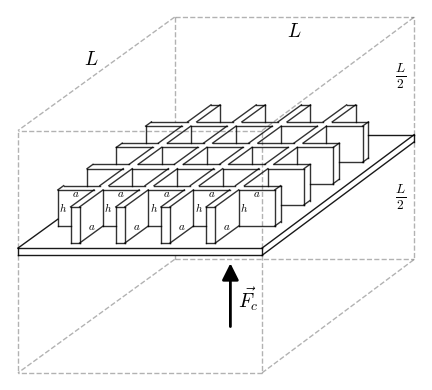
\includegraphics[width=0.48\textwidth]{honeycomb_box_L.png}
%\caption{}{Cubic cavity with a plate \\ covered by honeycomb}
%\end{center}
%\label{fig:honeycomb_box_L}
% \end{wrapfigure}

\vspace{\myvspacebeforesubsection}
    \subsection*{\centering{\fontencoding{T2A}\fontfamily{ptm}{\selectfont \uppercase{Двумерный подход Казимира}}}} \label{two-dimensional-casimirs-approach}
\vspace{\myvspaceaftersubsection}

% \begin{multicols}{2}

    Рассмотрим кубический резонатор объёмом \(L^3\), ограниченный идеально
проводящими стенками, в который помещена идеально проводящая квадратная пластина со стороной
\(L\), параллельная грани \(xy\), причём расстояние между пластиной и гранью \(xy\)
достаточно велико, например \(L/2\).
Одна сторона этой идеально проводящей квадратной пластины — гладкая плоскость, а
другая покрыта идеально проводящими сотами квадратной формы со стороной квадрата \(a\).

По обе стороны пластины выражения \(\sum\hbar\omega\big/2\)
где суммирование ведётся по всем возможным резонансным частотам резонатора \(L/2 \times L \times L\) (большой резонатор: между гладкой плоскостью и гранью \(xy\)) and the cavity \(L/2 \times a\times a\) (малый резонатор — одна ячейка сот: между дном соты и противоположной гранью \(xy\)) расходятся и лишены физического смысла, но разность этих сумм по противоположным сторонам пластины,
\(\left(\sum\,\,\hbar\omega\right)_{I}\big/{\left(2\,V_{I}\right)} - \left(\sum\,\,\hbar\omega\right)_{II}\big/{\left(2\,V_{II}\right)}\),
как будет показано, имеет вполне определённое значение, и это значение будет интерпретировано как взаимодействие между пластиной и обеими удалёнными гранями \(xy\).

    Возможные колебания внутри резонаторов, задаваемых условиями
\(0 \leq x \leq L\), \(0 \leq y \leq L\), \(0 \leq z \leq L/2\) (большой резонатор между гладкой плоскостью и гранью \(xy\))
и
\(0 \leq x \leq a\), \(0 \leq y \leq a\), \(0 \leq z \leq L/2\) (малый резонатор — одна ячейка сот) имеют волновые векторы
\(k_x = \frac{\pi}{L}\,n_x\), \(k_y = \frac{\pi}{L}\,n_y\),
\(k_z = \frac{\pi}{L/2}\,n_z\) (большой резонатор между гладкой плоскостью и гранью \(xy\)), а также
\(k_x = \frac{\pi}{a}\,n_x\), \(k_y = \frac{\pi}{a}\,n_y\),
\(k_z = \frac{\pi}{L/2}\,n_z\) (малый резонатор — одна ячейка сот),
где \(n_x\), \(n_y\), \(n_z\) — целые положительные числа;
    \(k = \sqrt{k_x^2+k_y^2+k_z^2} = \sqrt{\kappa^2+k_z^2}\).

\begin{figure}
\begin{center}
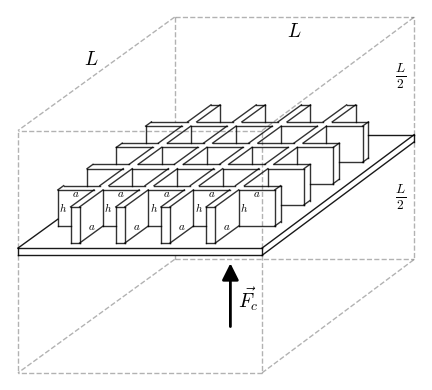
\includegraphics[width=0.42\textwidth]{honeycomb_box_L.png}
\caption{}{\centering{\textbf{Рис.1.} Кубический резонатор с пластиной, покрытой сотами.}}
\end{center}
\label{fig:honeycomb_box_L}
\end{figure}


Запишем выражение для суммы энергии нулевых колебаний в общем виде

\vspace{-3.5mm}
\begin{equation} \label{eq:1}
E = \frac{1}{2}\sum\,\hbar\omega = \hbar\,c\frac{1}{2}\sum\limits_{n_x}^{}\sum\limits_{n_y}^{}\sum\limits_{n_z}^{}k.
\end{equation}
\vspace{-3.5mm}

    Каждому набору \(k_x\), \(k_y\), \(k_z\) соответствуют две стоячие волны но если одно из \(n_i\) равно нулю, волна только одна.

    Для резонатора одной ячейки сот это несущественно по \(k_z\), поскольку при очень большом \(L/2\) можно считать \(k_z\) непрерывной переменной, заменив суммирование по \(n_z\) интегрированием.
Таким образом, для малого резонатора из одной соты находим

\noindent
\(E = \frac{\hbar\,c}{2}\int\limits_{0}^{\infty}\left[{\sqrt{k_z^2}+2\sum\limits_{n_x=1}^{\infty}\sum\limits_{n_y=1}^{\infty}\sqrt{\frac{n_x^2 \pi^2}{a^2}+\frac{n_y^2 \pi^2}{a^2}+k_z^2}}\right]d{n_z}\).

   Учитывая \(dn_z = \frac{L/2}{\pi}\,dk_z\) можно найти удельную плотность энергии \(E/V\), где
\(V = V_{small} = a^2 L/2\):

    % \(\frac{1}{2\,V}\sum\,\hbar\omega = \frac{\hbar\,c}{a^2\,L/2}\frac{1}{2}\int\limits_{0}^{\infty}\left[{\sqrt{k_z^2}+2\sum\limits_{n_x=1}^{\infty}\sum\limits_{n_y=1}^{\infty}\sqrt{n_x^2\frac{\pi^2}{a^2}+n_y^2\frac{\pi^2}{a^2}+k_z^2}}\right]\frac{L/2}{\pi}\,dk_z\)
% (small cavity, one honeycomb cell),

\noindent
\(\frac{E}{V} = \frac{\hbar\,c}{a^2\,\pi}\int\limits_{0}^{\infty}\left[{\frac{\sqrt{k_z^2}}{2}+\sum\limits_{n_x=1}^{\infty}\sum\limits_{n_y=1}^{\infty}\sqrt{\frac{n_x^2 \pi^2}{a^2}+\frac{n_y^2 \pi^2}{a^2}+k_z^2}}\right] dk_z\),
%(small cavity, one honeycomb cell),

\noindent
\(\frac{E}{V} = \frac{\hbar\,c}{a^2\,\pi}\int\limits_{0}^{\infty}\left[{\sum\limits_{n_x=(0)1}^{\infty}\sum\limits_{n_y=(0)1}^{\infty}\sqrt{n_x^2\frac{\pi^2}{a^2}+n_y^2\frac{\pi^2}{a^2}+k_z^2}}\right] dk_z\),
%(small cavity, one honeycomb cell),

    где обозначение \(\left(0\right) 1\) означает, что член с \(n_x = 0\) и \(n_y = 0\) следует умножить на \(1\big/2\). Таким образом, для малого резонатора из одной соты имеем

    \(\frac{E}{V} = \frac{\hbar\,c}{a^2\,\pi}\sum\limits_{n_x=(0)1}^{\infty}\sum\limits_{n_y=(0)1}^{\infty}\left[\int\limits_{0}^{\infty}\sqrt{n_x^2\frac{\pi^2}{a^2}+n_y^2\frac{\pi^2}{a^2}+k_z^2}\,dk_z\right]\).
%(small cavity, one honeycomb cell),

    Для большого резонатора это несущественно по \(k_x\), \(k_y\), поскольку при очень большом \(L\) можно считать \(k_x\), \(k_y\) непрерывными переменными. Таким образом, для большого резонатора между гладкой плоскостью и гранью \(xy\) находим
\noindent
\(\begin{array}{c}
\begin{array}{ll}
    \sum\frac{\hbar\omega}{2} = & \frac{\hbar c}{2}\int\limits_{0}^{\infty}\int\limits_{0}^{\infty}\Bigg[\sqrt{k_x^2+k_y^2}\,+ \\
   & +\,2\sum\limits_{n_z=1}^{\infty}\sqrt{\frac{n_z^2 \pi^2}{(L/2)^2}+k_x^2+k_y^2}\Bigg]d{n_x}d{n_y}.
\end{array}
\end{array}\)

%(large cavity between pure plane and \(xy\) face),

    При очень большом \(L/2\) последнее суммирование также можно заменить интегралом; следовательно, энергия большого резонатора равна

    \(\frac{1}{2}\sum\,\hbar\omega = \hbar\,c\int\limits_{0}^{\infty}\int\limits_{0}^{\infty}\int\limits_{0}^{\infty}\sqrt{k_z^2+k_x^2+k_y^2}\,d{n_x}\,d{n_y}\,d{n_z}\),
%(large cavity between pure plane and \(xy\) face),

    \(dn_x = \frac{L}{\pi}\,dk_x\), \(dn_y = \frac{L}{\pi}\,dk_y\),
\(dn_z = \frac{L/2}{\pi}\,dk_z\),

    Теперь для удельной плотности энергии \(E/V\) большого резонатора, где
\(V = V_{large} = L^3/2\) можно записать следующую цепочку преобразований:

\noindent
    \(\frac{E}{V} = \frac{\hbar\,c}{L^3/2}\int\limits_{0}^{\infty}\int\limits_{0}^{\infty}\int\limits_{0}^{\infty}\sqrt{k_z^2+k_x^2+k_y^2}\,dn_x\,dn_y\,\frac{L/2}{\pi}\,dk_z\),
%(large cavity between pure plane and \(xy\) face),

    % \(\frac{1}{2\,V}\sum\,\hbar\omega = \frac{\hbar\,c}{L^2\,\pi}\int\limits_{0}^{\infty}\int\limits_{0}^{\infty}\left[\,\int\limits_{0}^{\infty}\sqrt{k_z^2+k_x^2+k_y^2}\,dk_z\right]\,dn_x\,dn_y\)
% (large cavity between pure plane and \(xy\) face),
%\noindent
%    \(\frac{E}{V} = \frac{\hbar\,c}{L^2\,\pi}\int\limits_{0}^{\infty}\int\limits_{0}^{\infty}\left[\,\int\limits_{0}^{\infty}\sqrt{k_x^2+k_y^2+k_z^2}\,dk_z\right]\,dn_x\,dn_y\),
%(large cavity between pure plane and \(xy\) face),

\noindent
    \(\frac{E}{V} = \frac{\hbar\,c}{L^2\,\pi}\int\limits_{0}^{\infty}\int\limits_{0}^{\infty}\left[\,\int\limits_{0}^{\infty}\sqrt{k_x^2+k_y^2+k_z^2}\,dk_z\right]\,\left(\frac{L}{\pi}dk_x\right)\,\left(\frac{L}{\pi}dk_y\right)\),
%(large cavity between pure plane and \(xy\) face),

\noindent
    \(\frac{E}{V} = \frac{\hbar\,c}{a^2\,\pi}\int\limits_{0}^{\infty}\int\limits_{0}^{\infty}\left[\,\int\limits_{0}^{\infty}\sqrt{k_x^2+k_y^2+k_z^2}\,dk_z\right]\,\left(\frac{a}{\pi}dk_x\right)\,\left(\frac{a}{\pi}dk_y\right)\).
%(large cavity between pure plane and \(xy\) face),

И окончательно для большого резонатора между гладкой плоскостью и гранью \(xy\) плотность энергии можно записать так:

    \(\frac{\sum\,\hbar\omega}{2\,V} = \frac{\hbar\,c}{a^2\,\pi}\int\limits_{0}^{\infty}\int\limits_{0}^{\infty}\left[\,\int\limits_{0}^{\infty}\sqrt{k_x^2+k_y^2+k_z^2}\,dk_z\right]\,dn_x\,dn_y\),

а для малого резонатора, одной ячейки сот, имеем
\noindent
    \(\frac{\sum\,\hbar\omega}{2\,V} = \frac{\hbar\,c}{a^2\,\pi}\sum\limits_{n_x=(0)1}^{\infty}\sum\limits_{n_y=(0)1}^{\infty}\left[\,\int\limits_{0}^{\infty}\sqrt{n_x^2\frac{\pi^2}{a^2}+n_y^2\frac{\pi^2}{a^2}+k_z^2}\,dk_z\right]\).


%    \({\left(\frac{E}{V}\right)_{small\,cavity} = \frac{\hbar}{a^2} \sum\limits_{n_x=(0)1}^{\infty}\sum\limits_{n_y=(0)1}^{\infty}\,\int\limits_{0}^{\infty} {\frac {dk_{z}}{\pi}}\,\omega _{n_x,n_y},}\)

%    where
%\(\omega _{n_x,n_y} = c\,\sqrt{n_x^2\frac{\pi^2}{a^2}+n_y^2\frac{\pi^2}{a^2}+k_z^2}\)

Отсюда очевидно, что энергия взаимодействия определяется следующей разностью плотностей энергии:
%    \[\begin{array}{lr}
%\delta\,\frac{E}{V} =
%\begin{array}{c}
%\frac{\hbar\,c}{a^2\,\pi}\Bigg\{\sum\limits_{n_x=(0)1}^{\infty}\sum\limits_{n_y=(0)1}^{\infty}\left[\,\int\limits_{0}^{\infty}\sqrt{n_x^2\frac{\pi^2}{a^2}+n_y^2\frac{\pi^2}{a^2}+k_z^2}\,dk_z\right] - \\
%\int\limits_{0}^{\infty}\int\limits_{0}^{\infty}\left[\,\int\limits_{0}^{\infty}\sqrt{k_x^2+k_y^2+k_z^2}\,dk_z\right]\,\left(\frac{a}{\pi}dk_x\right)\,\left(\frac{a}{\pi}dk_y\right)\Bigg\}
%\end{array}\end{array}\]
\end{multicols}
\noindent

\vspace{-3.5mm}
    \begin{equation} \label{eq:2}
\begin{array}{lr}
\delta \frac{E}{V} =
\begin{array}{c}
\frac{\hbar c}{a^2 \pi}\Bigg\{\sum\limits_{n_x=(0)1}^{\infty}\sum\limits_{n_y=(0)1}^{\infty}\left[\int\limits_{0}^{\infty}\sqrt{\frac{n_x^2 \pi^2}{a^2}+\frac{n_y^2 \pi^2}{a^2}+k_z^2} dk_z\right] % \\ 
-\int\limits_{0}^{\infty}\int\limits_{0}^{\infty}\left[\int\limits_{0}^{\infty}\sqrt{k_x^2+k_y^2+k_z^2}\,dk_z\right] dn_x dn_y\Bigg\}.
\end{array}\end{array}\end{equation}
\vspace{-3.5mm}

\begin{multicols}{2}

    Это выражение явно бесконечно, и для продолжения расчёта удобно ввести регулятор.

    Чтобы получить конечный результат, подынтегральные выражения нужно умножить на регуляризующую функцию \(f(k/k_m)\), равную единице при \(k << k_m\) и достаточно быстро стремящуюся к нулю при \((k/k_m)\, \rightarrow\,\infty\). Здесь \(k_m\) можно определить условием \(f(1) = {1}/{2}\). Физический смысл очевиден: для очень коротких волн (например, рентгеновских) пластина практически не является препятствием, поэтому энергия нулевых колебаний этих волн не зависит от положения пластины.

    Регулятор нужен, чтобы сделать выражение конечным; влияние его конкретного вида в конце устраняется предельным переходом.

    Вводя переменную \(u^2 = a^2\,k_z^2/\pi^2\), \(du = a/\pi\,dk_z\), получаем:
\end{multicols}
\vspace{-3.5mm}
    \begin{equation} \label{eq:3}
\begin{array}{c}
\begin{array}{ll}
\delta\,\frac{E}{V} =
\frac{\hbar\,c\,\pi}{a^4}\Bigg\{
\sum\limits_{n_x=\left(0\right)\,1}^{\infty}
\sum\limits_{n_y=\left(0\right)\,1}^{\infty}
\int\limits_{0}^{\infty}
{\sqrt{n_x^2 + n_y^2 + u^2}} &
f\left(\frac{\pi\sqrt{n_x^2 + n_y^2 + u^2}}{a\,k_m}\right)
\,d{u} \\
\, &- \int\limits_{0}^{\infty}
\int\limits_{0}^{\infty}
\int\limits_{0}^{\infty}
{\sqrt{n_x^2 + n_y^2 + u^2}}
f\left(\frac{\pi\sqrt{n_x^2 + n_y^2 + u^2}}{a\,k_m}\right)
\,d{u}\,d{n_x}\,d{n_y}
\Bigg\}.
\end{array}
\end{array}
\end{equation}
\vspace{-3.5mm}
\begin{multicols}{2}
    Если \(\omega _{n_x,n_y} = c\,\sqrt{n_x^2\frac{\pi^2}{a^2}+n_y^2\frac{\pi^2}{a^2}+k_z^2}\)
и \(k_z^2 = u^2 \frac{\pi^2}{a^2}\), то
\(\omega _{n_x,n_y} = c \, \frac{\pi}{a} \sqrt{n_x^2+n_y^2+u^2}\), так что
\(f\left(\frac{\pi\sqrt{n_x^2 + n_y^2+u^2}}{a\,k_m}\right) = f\left(\frac{\omega _{n_x,n_y}}{c\,k_m}\right)\),
где частота обрезания \(\omega_m = c\,k_m\).
    Вводя функцию
\noindent
\begin{equation} \label{eq:4}
F = %\left(u, n_x, n_y\right) =
\sqrt{n_x^2 + n_y^2+u^2}\,
f\left(\frac{\pi\sqrt{n_x^2 + n_y^2+u^2}}{a\,k_m}\right)
\end{equation}

    можно записать

\noindent
$\begin{array}{c}
\begin{array}{ll}
\delta\,\frac{E}{V} =
\frac{\hbar\,c\,\pi}{a^4}
&\Bigg\{
\sum\limits_{n_x=\left(0\right)\,1}^{\infty}
\sum\limits_{n_y=\left(0\right)\,1}^{\infty}
\left(\int\limits_{0}^{\infty}F\left(u, n_x, n_y\right)\,d{u}\right)
\\
\, & \,\,\,\,\,\, - \int\limits_{0}^{\infty}
\int\limits_{0}^{\infty}
\left(\int\limits_{0}^{\infty}F\left(u, n_x, n_y\right)\,d{u}\right)
\,d{n_x}\,d{n_y}
\Bigg\}.
\end{array}
\end{array}$

    И, наконец, вводя
\noindent
\begin{equation} \label{eq:5}
G\left(n_x, n_y\right) = \int\limits_{0}^{\infty}F\left(u, n_x, n_y\right)\,d{u}
\end{equation}

    имеем
    \begin{equation} \label{eq:6}
\begin{array}{lr}
\delta\,\frac{E}{V} =
\begin{array}{c}
 \frac{\hbar\,c\,\pi}{a^4} \Bigg\{
\sum\limits_{n_x=\left(0\right)\,1}^{\infty}
\sum\limits_{n_y=\left(0\right)\,1}^{\infty}
G\left(n_x, n_y\right)
\\
- \int\limits_{0}^{\infty}
\int\limits_{0}^{\infty}
G\left(n_x, n_y\right)
\,d{n_x}\,d{n_y}
\Bigg\}.
\end{array}
\end{array}
\end{equation}

Интегрирование \(G\left(n_x, n_y\right)\) с примером регуляризующей функции приведено в приложении A.

    Для получения способа вычисления \(\delta\left(E/V\right)\) можно воспользоваться двумерной формулой Эйлера–Маклорена.

% \end{multicols}

\vspace{\myvspacebeforesubsection}
\subsection*{\centering{\fontencoding{T2A}\fontfamily{ptm}{\selectfont \uppercase{Двумерная формула Эйлера–Маклорена}}}} \label{eulermaclaurin-2d-formula}
\vspace{\myvspaceaftersubsection}

% \begin{multicols}{2}

Следуя А.~Бикялису \cite{Bikyalis1968}, применим формулу Эйлера–Маклорена дважды — по \(n_x\) и по \(n_y\), исходя из следующей её формы

% \[{\displaystyle \sum _{i=a}^{b}f(i)=\int\limits_{a}^{b}f(x)\,dx+{\frac {f(a)+f(b)}{2}}+\sum\limits_{k=1}^{\lfloor p/2\rfloor }{\frac {B_{2k}}{(2k)!}}\left(f^{(2k-1)}(b)-f^{(2k-1)}(a)\right)+R_{p},}\]

    \begin{equation} \label{eq:7}
\begin{array}{l}
\begin{array}{ll}
\displaystyle \sum _{i=a}^{b}f(i)= \int_{a}^{b}f(x)\,dx+{\frac {f(a)+f(b)}{2}} + & \,\,\,\,
\end{array}  \\
\begin{array}{rr}
\,\,\, & +\,\sum_{k=1}^{\lfloor p/2\rfloor }{\frac {B_{2k}}{(2k)!}}\left(f^{(2k-1)}(b)-f^{(2k-1)}(a)\right)+ \\
\,\,\, & + \,R_{p},
\end{array}
\end{array}\end{equation}

\begin{equation} \label{eq:8}
{\displaystyle P_{k}(x)=B_{k}\left(x-\lfloor x\rfloor \right),}
\end{equation}

\begin{equation} \label{eq:9}
{\displaystyle R_{p}=(-1)^{p+1}\int_{a}^{b}f^{(p)}(x){\frac {P_{p}(x)}{p!}}\,dx},
\end{equation}

поскольку мы имеем дело с очень сложной математической задачей интегрирования функции, которая часто осциллирует и терпит разрывы в точках каждого целого значения аргумента из-за множителя \((x-\lfloor x\rfloor )\), далее будем использовать то, что остаточный член можно записать также в виде

\begin{equation} \label{eq:10}
{\displaystyle R_{p}=(-1)^{p+1}\sum_{j=a}^{b-1} \int _{0}^{1}f^{(p)}(v+j){\frac {B_{p}(v)}{p!}}\,dv}.
\end{equation}

Видно, что формула состоит из 4 частей:

\noindent
интеграл \(\int\limits_{x}^{}=\int _{x_a}^{x_b}f(x)\,dx\),

\noindent
полусумма \(\underset{x}{H_{\sum}}={\left( {f(x_a)+f(x_b)}\right)/{2}}\),

\noindent
сумма полиномов Бернулли

\({\sum\limits_{x}^{}}^{B}=\sum _{k=1}^{\lfloor p/2\rfloor }{\frac {B_{2k}}{(2k)!}}\left(f^{(2k-1)}(x_b)-f^{(2k-1)}(x_a)\right)\),

\noindent
и остаточный член

\(\underset{x}{R_{p}}=(-1)^{p+1}\sum_{j=x_a}^{x_b-1} \int _{0}^{1}f^{(p)}(v_x+j_x){\frac {B_{p}(v_x)}{p!}}\,dv_x\).

Применяя её к \(G\) дважды — по \(n_x\) и по \(n_y\), — получаем следующие слагаемые, которые можно представить таблицей:

    \begin{equation} \label{eq:11}
\begin{array}{cccc}
 \int\limits_{n_y}^{} \int\limits_{n_x}^{} G  &  \int\limits_{n_y}^{} \underset{n_x}{H_{\sum}}\,G  &  \int\limits_{n_y}^{}{\sum\limits_{n_x}^{}}^{B}\,G  &  \int\limits_{n_y}^{}\,\underset{n_x}{R_{p}}\,G  \\
 \underset{n_y}{H_{\sum}}\,\int\limits_{n_x}^{}\,G &  \underset{n_y}{H_{\sum}}\,\underset{n_x}{H_{\sum}}\,G &  \underset{n_y}{H_{\sum}}\,{\sum\limits_{n_x}^{}}^{B}\,G &  \underset{n_y}{H_{\sum}}\,\underset{n_x}{R_{p}}\,G \\
 {\sum\limits_{n_y}^{}}^{B}\,\int\limits_{n_x}^{}\,G  &  {\sum\limits_{n_y}^{}}^{B}\,\underset{n_x}{H_{\sum}}\,G  &  {\sum\limits_{n_y}^{}}^{B}\,{\sum\limits_{n_x}^{}}^{B}\,G  &  {\sum\limits_{n_y}^{}}^{B}\,\underset{n_x}{R_{p}}\,G  \\
 \underset{n_y}{R_{p}}\,\int\limits_{n_x}^{}\,G   &  \underset{n_y}{R_{p}}\,\underset{n_x}{H_{\sum}}\,G   &  \underset{n_y}{R_{p}}\,{\sum\limits_{n_x}^{}}^{B}\,G   &  \underset{n_y}{R_{p}}\,\underset{n_x}{R_{p}}\,G.
\end{array}\end{equation}

    Поскольку функция \(G\) симметрична по аргументам \(n_x\) и \(n_y\), приведённая выше двумерная матрица Эйлера–Маклорена также симметрична.

% \end{multicols}

\vspace{\myvspacebeforesubsection}
    \subsection*{\centering{\fontencoding{T2A}\fontfamily{ptm}{\selectfont \uppercase{Итоги двумерной формулы Эйлера–Маклорена}}}} \label{summary-of-eulermaclaurin-2d}
\vspace{\myvspaceaftersubsection}

% \begin{multicols}{2}

При значении параметра \(p = 1\) имеем:

    \begin{center}
\begin{tabular}{ l }
%\hline

$\int\limits_{n_y}^{} \int\limits_{n_x}^{} G = \int\limits_{a_{y}}^{b_{y}} \int\limits_{a_{x}}^{b_{x}} G\left(n_{x}, n_{y}\right)\,{d n_{x}}\,{d n_{y}}$ \\

$\int\limits_{n_y}^{} \underset{n_x}{H_{\sum}}\,G = \frac{1}{2} \, \int\limits_{a_{y}}^{b_{y}} G\left(a_{x}, n_{y}\right)\,{d n_{y}}$ \\

$\int\limits_{n_y}^{} {\sum\limits_{n_x}^{}}^{B}\,G = 0$ \\

$\int\limits_{n_y}^{} \underset{n_x}{R_{p}}\,G = {\sum\limits_{j_{x}=a_{x}}^{b_{x} - 1} \int\limits_{a_{y}}^{b_{y}} \int\limits_{0}^{1} \frac{1}{2} \, {\left(2 \, v_{n_{x}} - 1\right)} G'\left(\widehat{j_{x} + v_{n_{x}}}, n_{y}\right){d v_{n_{x}}}{d n_{y}}}$ \\

%\hline

\end{tabular}
\end{center}

    \begin{center}
\begin{tabular}{ l }

%\hline

$\underset{n_y}{H_{\sum}}\,\int\limits_{n_x}^{}\,G = \frac{1}{2} \, \int\limits_{a_{x}}^{b_{x}} G\left(n_{x}, a_{y}\right)\,{d n_{x}}$ \\

$\underset{n_y}{H_{\sum}}\,\underset{n_x}{H_{\sum}}\,G = \frac{1}{4} \, G\left(a_{x}, a_{y}\right)$ \\

$\underset{n_y}{H_{\sum}}\,{\sum\limits_{n_x}^{}}^{B}\,G = 0$ \\

$\underset{n_y}{H_{\sum}}\,\underset{n_x}{R_{p}}\,G = {\sum\limits_{j_{n_{x}}=a_{x}}^{b_{x} - 1} \frac{1}{4} \, \int\limits_{0}^{1} \left(2 \, v_{n_{x}} - 1 \right) G'\left(\widehat{j_{n_{x}} + v_{n_{x}}}, a_{y}\right)\,{d v_{n_{x}}} }$ \\

%\hline

\end{tabular}
\end{center}

    \begin{center}
\begin{tabular}{ l }

%\hline

${\sum\limits_{n_y}^{}}^{B}\,\int\limits_{n_x}^{}\,G = 0$ \\

${\sum\limits_{n_y}^{}}^{B}\,\underset{n_x}{H_{\sum}}\,G = 0$ \\

${\sum\limits_{n_y}^{}}^{B}\,{\sum\limits_{n_x}^{}}^{B}\,G = 0$ \\

${\sum\limits_{n_y}^{}}^{B}\,\underset{n_x}{R_{p}}\,G = 0$ \\

%\hline

\end{tabular}
\end{center}

    \begin{center}
\begin{tabular}{ l }

%\hline

$\underset{n_y}{R_{p}}\,\int\limits_{n_x}^{}\,G = {\sum\limits_{j_{x}=a_{x}}^{b_{x} - 1} \int\limits_{a_{y}}^{b_{y}} \int\limits_{0}^{1} \frac{1}{2} \, {\left(2 \, v_{n_{x}} - 1\right)} G'\left(\widehat{j_{x} + v_{n_{x}}}, n_{y}\right){d v_{n_{x}}}{d n_{y}}}$ \\

$\underset{n_y}{R_{p}}\,\underset{n_x}{H_{\sum}}\,G = {\sum\limits_{j_{n_{y}}=a_{y}}^{b_{y} - 1} \int\limits_{0}^{1} \frac{1}{4} \, {\left(2 \, v_{n_{y}} - 1\right)} G'\left(a_{x}, \widehat{j_{n_{y}} + v_{n_{y}}}\right)\,{d v_{n_{y}}}}$ \\

$\underset{n_y}{R_{p}}\,{\sum\limits_{n_x}^{}}^{B}\,G = 0$ \\

%$\underset{n_y}{R_{p}}\,\underset{n_x}{R_{p}}\,G = {\sum\limits_{j_{y}=a_{y}}^{b_{y} - 1} {\sum\limits_{j_{x}=a_{x}}^{b_{x} - 1} \int\limits_{0}^{1} \int\limits_{0}^{1}\frac{1}{4} {\left(2 \, v_{y} - 1\right)} {\left(2 \, v_{x} - 1\right)} 
%G''\left(\widehat{j_{x} + v_{x}}, \widehat{j_{y} + v_{y}}\right)\,{d v_{x}}}\,{d v_{y}}}$ \\


$\begin{array}{lr}
\underset{n_y}{R_{p}}\,\underset{n_x}{R_{p}}\,G =
\begin{array}{c}
 \sum\limits_{j_{y}=a_{y}}^{b_{y} - 1} \sum\limits_{j_{x}=a_{x}}^{b_{x} - 1} \int\limits_{0}^{1} \int\limits_{0}^{1}\frac{1}{4} \left(2 \, v_{y} - 1\right)  \left(2 \, v_{x} - 1\right) \cdot \\
G''\left(\widehat{j_{x} + v_{x}}, \widehat{j_{y} + v_{y}}\right)\,{d v_{x}}\,{d v_{y}}
\end{array}
\end{array}$ \\


%\hline

\end{tabular}
\end{center}

% \end{multicols}

\vspace{\myvspacebeforesubsection}
    \subsection*{\centering {\fontencoding{T2A}\fontfamily{ptm}{\selectfont {\uppercase{Способ \\ вычисления~}\(\delta\left(E/V\right)\)}}}}\label{a-way-of-calculating-deltaleftevright}
\vspace{\myvspaceaftersubsection}

% \begin{multicols}{2}

    Рассмотрим выражение

\begin{equation} \label{eq:12}
\sum\limits_{n_x=\left(0\right)\,1}^{\infty}
\sum\limits_{n_y=\left(0\right)\,1}^{\infty}
G%\left(n_x, n_y\right)
-
\int\limits_{0}^{\infty}
\int\limits_{0}^{\infty}
G%\left(n_x, n_y\right)
\,\,\,d{n_x}\,d{n_y}
\end{equation}

    Во-первых, видно, что

\begin{equation} \label{eq:13}
\begin{array}{c}
    \sum\limits_{n_x=\left(0\right)\,1}^{\infty} \sum\limits_{n_y=\left(0\right)\,1}^{\infty} {G\left(n_x, n_y\right)} = \\
% \sum\limits_{n_x=\left(0\right)\,1}^{\infty} \left( -\frac{1}{2}G\left(n_x, 0\right) + \sum\limits_{n_y=0}^{\infty}{G\left(n_x, n_y\right)} \right) = \\
% -\frac{1}{2} \left( -\frac{1}{2}G\left(0, 0\right) + \sum\limits_{n_y=0}^{\infty}{G\left(0, n_y\right)} \right) + \\
%\sum\limits_{n_x=0}^{\infty} \left( -\frac{1}{2}G\left(n_x, 0\right) + \sum\limits_{n_y=0}^{\infty}{G\left(n_x, n_y\right)} \right) = \\
 \frac{1}{4}G\left(0, 0\right) - \frac{1}{2}\sum\limits_{n_y=0}^{\infty}{G\left(0, n_y\right)}\, - \\
\frac{1}{2}\sum\limits_{n_x=0}^{\infty}{G\left(n_x, 0\right)} + \sum\limits_{n_x=0}^{\infty}\sum\limits_{n_y=0}^{\infty}{G\left(n_x, n_y\right)}.
\end{array}
\end{equation}

    Следовательно, имеем

\noindent
\(\begin{array}{l}
\begin{array}{ll}
\sum\limits_{n_x=\left(0\right)\,1}^{\infty} \sum\limits_{n_y=\left(0\right)\,1}^{\infty} G\left(n_x, n_y\right)
 - \\
\,\,\,\,\,\,\,\,\,\,\,\,\,\,\,\,\,\,\,\,\,\,\,\,\,\,\,\,\,\,\,\,\,\,\,\,\,\,\,\,\,\,\,\,\,\,\,\,\,\,\,\int\limits_{0}^{\infty} \int\limits_{0}^{\infty} G\left(n_x, n_y\right)\,d{n_x}\,d{n_y} = & \, \\
\end{array} \\
\begin{array}{c}
\frac{1}{4}G\left(0, 0\right) -\frac{1}{2}\sum\limits_{n_y=0}^{\infty}{G\left(0, n_y\right)} -\frac{1}{2}\sum\limits_{n_x=0}^{\infty}{G\left(n_x, 0\right)}\, + \\
\end{array} \\
\begin{array}{rr}
\, & \sum\limits_{n_x=0}^{\infty}\sum\limits_{n_y=0}^{\infty}{G\left(n_x, n_y\right)} - \int\limits_{0}^{\infty} \int\limits_{0}^{\infty} G\left(n_x, n_y\right)\,d{n_x}\,d{n_y}.
\end{array}
\end{array}\)

    С другой стороны, мы нашли, что

\noindent
\(\sum\limits_{n_x=0}^{\infty} \sum\limits_{n_y=0}^{\infty} G\left(n_x, n_y\right) -\int\limits_{0}^{\infty} \int\limits_{0}^{\infty} G\left(n_x, n_y\right)\,d{n_x}\,d{n_y} = \\
 \begin{array}{cccc}  \, &  \int\limits_{n_y}^{} \underset{n_x}{H_{\sum}}\,G &  + \int\limits_{n_y}^{}{\sum\limits_{n_x}^{}}^{B}\,G &  + \int\limits_{n_y}^{}\,\underset{n_x}{R_{p}}\,G \\
  +\underset{n_y}{H_{\sum}}\,\int\limits_{n_x}^{}\,G &  + \underset{n_y}{H_{\sum}}\,\underset{n_x}{H_{\sum}}\,G &  + \underset{n_y}{H_{\sum}}\,{\sum\limits_{n_x}^{}}^{B}\,G &  + \underset{n_y}{H_{\sum}}\,\underset{n_x}{R_{p}}\,G \\
  + {\sum\limits_{n_y}^{}}^{B}\,\int\limits_{n_x}^{}\,G &  + {\sum\limits_{n_y}^{}}^{B}\,\underset{n_x}{H_{\sum}}\,G &  + {\sum\limits_{n_y}^{}}^{B}\,{\sum\limits_{n_x}^{}}^{B}\,G &  + {\sum\limits_{n_y}^{}}^{B}\,\underset{n_x}{R_{p}}\,G \\
  + \underset{n_y}{R_{p}}\,\int\limits_{n_x}^{}\,G &  + \underset{n_y}{R_{p}}\,\underset{n_x}{H_{\sum}}\,G &  + \underset{n_y}{R_{p}}\,{\sum\limits_{n_x}^{}}^{B}\,G &  + \underset{n_y}{R_{p}}\,\underset{n_x}{R_{p}}\,G, \end{array}\)

    где \(\underset{n_y}{H_{\sum}}\,\underset{n_x}{H_{\sum}}\,G\),
\(\int\limits_{n_y}^{} \underset{n_x}{H_{\sum}}\,G\)
и
\(\underset{n_y}{H_{\sum}}\,\int\limits_{n_x}^{}\,G\) равны:

\noindent
    \(\frac{1}{4} \, G\left(a_{x}, a_{y}\right) , \frac{1}{2} \, \int_{a_{y}}^{b_{y}} G\left(a_{x}, n_{y}\right)\,{d n_{y}} , \frac{1}{2} \, \int_{a_{x}}^{b_{x}} G\left(n_{x}, a_{y}\right)\,{d n_{x}}.\)

    Теперь, используя одномерную формулу Эйлера–Маклорена в виде (\ref{eq:7}), видим, что

%\noindent
%$\begin{array}{l}
%\begin{array}{ll}
%\displaystyle \sum _{i=a}^{b}f(i)=\int _{a}^{b}f(x)\,dx+{\frac {f(a)+f(b)}{2}}+ & \, \\
%\end{array} \\
%\begin{array}{rr}
%\, &
%\sum _{k=1}^{\lfloor p/2\rfloor }{\frac {B_{2k}}{(2k)!}}(f^{(2k-1)}(b)-f^{(2k-1)}(a))+R_{p},
%\end{array}
%\end{array}$

    

    \[
\frac{1}{4}G\left(0, 0\right)
- \frac{1}{2}\sum\limits_{n_y=0}^{\infty}{G\left(0, n_y\right)}
- \frac{1}{2}\sum\limits_{n_x=0}^{\infty}{G\left(n_x, 0\right)}
\]

    будет равно

\noindent
\(\begin{array}{l}
    \begin{array}{l}
  \underset{n_y}{H_{\sum}} \underset{n_x}{H_{\sum}} G \\
\end{array} \\
\begin{array}{rrrrr}
  \, &  - \int\limits_{n_y}^{} \underset{n_x}{H_{\sum}}\,G &  - \underset{n_y}{H_{\sum}} \underset{n_x}{H_{\sum}}\,G &  - \frac{1}{2}{\sum\limits_{n_y}^{}}^{B}\,G &  - \frac{1}{2}\underset{n_y}{R_{p}}\,G/2 \\
  \,&  - \underset{n_y}{H_{\sum}}\int\limits_{n_x}^{} \,G &  - \underset{n_y}{H_{\sum}} \underset{n_x}{H_{\sum}}\,G &  - \frac{1}{2}{\sum\limits_{n_x}^{}}^{B}\,G &  - \frac{1}{2}\underset{n_x}{R_{p}}\,G/2. \\
\end{array}
\end{array}\)

    Теперь выражение (\ref{eq:12}) можно найти следующим суммированием

%\(\sum\limits_{n_x=\left(0\right)\,1}^{\infty} \sum\limits_{n_y=\left(0\right)\,1}^{\infty} G\left(n_x, n_y\right) - \int\limits_{0}^{\infty} \int\limits_{0}^{\infty} G\left(n_x, n_y\right)\,d{n_x}\,d{n_y}\)



\noindent
    \(\begin{array}{llll}  \,&  \,&  + \int\limits_{n_y}^{}{\sum\limits_{n_x}^{}}^{B}\,G &  + \int\limits_{n_y}^{}\,\underset{n_x}{R_{p}}\,G \\  \,&  \,&  + \underset{n_y}{H_{\sum}}\,{\sum\limits_{n_x}^{}}^{B}\,G &  + \underset{n_y}{H_{\sum}}\,\underset{n_x}{R_{p}}\,G \\  + {\sum\limits_{n_y}^{}}^{B}\,\int\limits_{n_x}^{}\,G &  + {\sum\limits_{n_y}^{}}^{B}\,\underset{n_x}{H_{\sum}}\,G &  + {\sum\limits_{n_y}^{}}^{B}\,{\sum\limits_{n_x}^{}}^{B}\,G &  + {\sum\limits_{n_y}^{}}^{B}\,\underset{n_x}{R_{p}}\,G \\  + \underset{n_y}{R_{p}}\,\int\limits_{n_x}^{}\,G &  + \underset{n_y}{R_{p}}\,\underset{n_x}{H_{\sum}}\,G &  + \underset{n_y}{R_{p}}\,{\sum\limits_{n_x}^{}}^{B}\,G &  + \underset{n_y}{R_{p}}\,\underset{n_x}{R_{p}}\,G \\  \,&  \,&  - \frac{1}{2}{\sum\limits_{n_y}^{}}^{B}\,G &  - \frac{1}{2}\underset{n_y}{R_{p}}\,G \\  \,&  \,&  - \frac{1}{2}{\sum\limits_{n_x}^{}}^{B}\,G &  - \frac{1}{2}\underset{n_x}{R_{p}}\,G. \\ \end{array}\)

    Легко видеть, что сумма всех слагаемых без остаточных членов

    \(\begin{array}{llll}  \,&  \,&  + \int\limits_{n_y}^{}{\sum\limits_{n_x}^{}}^{B}\,G \\  \,&  \,&  + \underset{n_y}{H_{\sum}}\,{\sum\limits_{n_x}^{}}^{B}\,G \\  + {\sum\limits_{n_y}^{}}^{B}\,\int\limits_{n_x}^{}\,G &  + {\sum\limits_{n_y}^{}}^{B}\,\underset{n_x}{H_{\sum}}\,G &  + {\sum\limits_{n_y}^{}}^{B}\,{\sum\limits_{n_x}^{}}^{B}\,G\\  \,&  \,&  - \frac{1}{2}{\sum\limits_{n_y}^{}}^{B}\,G \\  \,&  \,&  - \frac{1}{2}{\sum\limits_{n_x}^{}}^{B}\,G \\ \end{array}\)

    равна 0. Следовательно, любой возможный ненулевой результат выражения (\ref{eq:12}) следует отнести к остаточному члену
\noindent
    \(\begin{array}{r} \sum\limits_{n_x=\left(0\right)\,1}^{\infty} \sum\limits_{n_y=\left(0\right)\,1}^{\infty} G\left(n_x, n_y\right) - \int\limits_{0}^{\infty} \int\limits_{0}^{\infty} G\left(n_x, n_y\right)\,d{n_x}\,d{n_y} = \end{array}\)

    \(\begin{array}{llll}  \,&  \,&  \,&  + \int\limits_{n_y}^{}\,\underset{n_x}{R_{p}}\,G \\  \,&  \,&  \,&  + \underset{n_y}{H_{\sum}}\,\underset{n_x}{R_{p}}\,G \\  \,&  \,&  \,&  + {\sum\limits_{n_y}^{}}^{B}\,\underset{n_x}{R_{p}}\,G \\  + \underset{n_y}{R_{p}}\,\int\limits_{n_x}^{}\,G &  + \underset{n_y}{R_{p}}\,\underset{n_x}{H_{\sum}}\,G &  + \underset{n_y}{R_{p}}\,{\sum\limits_{n_x}^{}}^{B}\,G &  + \underset{n_y}{R_{p}}\,\underset{n_x}{R_{p}}\,G \\  \,&  \,&  \,&  - \frac{1}{2}\underset{n_y}{R_{p}}\,G \\  \,&  \,&  \,&  - \frac{1}{2}\underset{n_x}{R_{p}}\,G. \\ \end{array}\)

    Или, используя симметрию \(G\), можно переписать итоговую формулу

\noindent
    \(\begin{array}{r} \sum\limits_{n_x=\left(0\right)\,1}^{\infty} \sum\limits_{n_y=\left(0\right)\,1}^{\infty} G\left(n_x, n_y\right) - \int\limits_{0}^{\infty} \int\limits_{0}^{\infty} G\left(n_x, n_y\right) d{n_x} d{n_y} = \end{array}\)

    \(\begin{array}{rr}
\, & +\,2\cdot\underset{n_y}{R_{p}}\,\int\limits_{n_x}^{}\,G +\,2\cdot\underset{n_y}{R_{p}}\,\underset{n_x}{H_{\sum}}\,G +\,2\cdot\underset{n_y}{R_{p}}\,{\sum\limits_{n_x}^{}}^{B}\,G\,+ \\
\, & +\,\underset{n_y}{R_{p}}\,\underset{n_x}{R_{p}}\,G -\,\underset{n_y}{R_{p}}\,G
\end{array}\)

    со следующими слагаемыми:

\noindent
\(2 \underset{n_y}{R_{p}}\int\limits_{n_x}^{} G = {\sum\limits_{j_{x}=a_{x}}^{b_{x} - 1} \int\limits_{a_{y}}^{b_{y}} \int\limits_{0}^{1} {\left(2 v_{n_{x}} - 1\right)} G'\left(\widehat{j_{x} + v_{n_{x}}}, n_{y}\right) {d v_{n_{x}}} {d n_{y}}}\);

\noindent
\(2 \underset{n_y}{R_{p}}\underset{n_x}{H_{\sum}} G = {\sum\limits_{j_{n_{y}}=a_{y}}^{b_{y} - 1} \int\limits_{0}^{1}  {\left(v_{n_{y}} - \frac{1}{2}\right)}\,G'\left(a_{x}, \widehat{j_{n_{y}} + v_{n_{y}}}\right) {d v_{n_{y}}}}\);

\(2 \underset{n_y}{R_{p}}{\sum\limits_{n_x}^{}}^{B}\,G = 2 {\sum\limits_{j_{n_{y}}=a_{y}}^{b_{y} - 1} \int\limits_{0}^{1} 0\,{d v_{n_{y}}}} = 0\);

%\(\underset{n_y}{R_{p}}\,\underset{n_x}{R_{p}}G = {\sum\limits_{j_{y}=a_{y}}^{b_{y} - 1} {\sum\limits_{j_{x}=a_{x}}^{b_{x} - 1} \int\limits_{0}^{1} \int\limits_{0}^{1} \frac{1}{4} \, {\left(2 \, v_{y} - 1\right)} {\left(2 \, v_{x} - 1\right)} G''\left(\widehat{j_{x} + v_{x}}, \widehat{j_{y} + v_{y}}\right)\,{d v_{x}}}\,{d v_{y}}}\)

\noindent
$\begin{array}{lr}
\underset{n_y}{R_{p}}\,\underset{n_x}{R_{p}}\,G =
\begin{array}{c}
 \sum\limits_{j_{y}=a_{y}}^{b_{y} - 1} \sum\limits_{j_{x}=a_{x}}^{b_{x} - 1} \int\limits_{0}^{1} \int\limits_{0}^{1} \left(v_{y} - \frac{1}{2}\right)  \left(v_{x} - \frac{1}{2}\right) \\
\cdot \, G''\left(\widehat{j_{x} + v_{x}}, \widehat{j_{y} + v_{y}}\right)\,{d v_{x}}\,{d v_{y}};
\end{array}
\end{array}$

\noindent
\(-\underset{n_y}{R_{p}}\,G = -{\sum\limits_{j_{n_{y}}=a_{y}}^{b_{y} - 1} \int\limits_{0}^{1} {\left(v_{n_{y}} - \frac{1}{2}\right)}\,G'\left(n_{x}, \widehat{j_{n_{y}} + v_{n_{y}}}\right)\,{d v_{n_{y}}}}\).

    Учитывая, что \(\underset{n_y}{R_{p}}\,{\sum\limits_{n_x}^{}}^{B}\,G\)
должно равняться \(0\), поскольку производная по \(n_x\) при \(n_x = 0\) равна \(0\), а
\(\,2\cdot\underset{n_y}{R_{p}}\,\underset{n_x}{H_{\sum}}\,G -\,\underset{n_y}{R_{p}}\,G\)
в сумме даёт \(0\), результат можно упростить до вида

\end{multicols}
\vspace{-3.5mm}

    \begin{equation}
\begin{array}{r}
\sum\limits_{n_x=\left(0\right)\,1}^{\infty}
\sum\limits_{n_y=\left(0\right)\,1}^{\infty}
G\left(n_x, n_y\right)
-
\int\limits_{0}^{\infty}
\int\limits_{0}^{\infty}
G\left(n_x, n_y\right)\,d{n_x}\,d{n_y} =
\,2\cdot\underset{n_y}{R_{p}}\,\int\limits_{n_x}^{}\,G 
+\,\underset{n_y}{R_{p}}\,\underset{n_x}{R_{p}}\,G
\end{array}
\end{equation}

    или в развёрнутом виде

\noindent
\begin{equation}
\begin{array}{r}
\sum\limits_{n_x=\left(0\right)\,1}^{\infty}
\sum\limits_{n_y=\left(0\right)\,1}^{\infty}
G%\left(n_x, n_y\right)
-
\int\limits_{0}^{\infty}
\int\limits_{0}^{\infty}
G%\left(n_x, n_y\right)
\,\,\, d{n_x} d{n_y}  =
{\sum\limits_{j_{x}=0}^{\infty} \int\limits_{n_{y}=0}^{\infty} \int\limits_{v_x=0}^{1}  {\left(2 \, v_{n_{x}} - 1\right)}\, G'\left(\widehat{j_{x} + v_{n_{x}}}, n_{y}\right) {d v_{n_{x}}} {d n_{y}}} \, + \\
 + \,\sum\limits_{j_{y}=0}^{\infty} \sum\limits_{j_{x}=0}^{\infty} \int\limits_{0}^{1} \int\limits_{0}^{1} {\left(v_{y} - \frac{1}{2}\right)} {\left(v_{x} - \frac{1}{2}\right)} \, G''\left(\widehat{j_{x} + v_{x}}, \widehat{j_{y} + v_{y}}\right){d v_{x}}{d v_{y}}.
\end{array}
\end{equation}

\begin{multicols}{2}

% \end{multicols}

\vspace{\myvspacebeforesubsection}
    \subsection*{\centering {\fontencoding{T2A}\fontfamily{ptm}{\selectfont {\uppercase{Как} \(\delta\left(E/V\right)\) \\ \uppercase{зависит от} \(a k_m\)?}}}} \label{how-deltaleftevright-depends-on-a-k_m}
\vspace{\myvspaceaftersubsection}

% \begin{multicols}{2}

    Казимир в исходной работе \cite{Casimir1948} получил свою формулу в предположении \(a\,k_m\,>>\,1\). Теперь же можно исследовать, как выражение (\ref{eq:12}) зависит от \(a k_m\).

%\(\sum\limits_{n_x=\left(0\right)\,1}^{\infty} \sum\limits_{n_y=\left(0\right)\,1}^{\infty} G\left(n_x, n_y\right) - \int\limits_{0}^{\infty} \int\limits_{0}^{\infty} G\left(n_x, n_y\right)\,d{n_x}\,d{n_y}\)

    Таким образом, для разности плотностей энергии на \(cm^2\) находим

\vspace{-3.5mm}
\begin{equation}
\begin{array}{r}
    \delta\,\frac{E}{V} = \frac{\hbar\,c\,\pi}{a^4} \int\limits_{0}^{\infty} \Bigg\{ \sum\limits_{n_x=\left(0\right)\,1}^{\infty} \sum\limits_{n_y=\left(0\right)\,1}^{\infty} F\left(n_x, n_y\right) \,\,\,\,\,\,\,\,\,\,\\ 
- \int\limits_{0}^{\infty} \int\limits_{0}^{\infty} F\left(n_x, n_y\right) d{n_x} d{n_y} \Bigg\} d{u}.
\end{array}
\end{equation}

\vspace{-3.5mm}

\noindent
\begin{center}
\begin{tabular}{ r }
Таблица 1. Результат вычисления выражения (\ref{eq:12}).
\end{tabular}

\vspace{+3.5mm}

\begin{tabular}{ | l | c | c | c | }
\hline
$a \cdot k_m$ & $\sum\limits_{\left(0\right)\,1}^{\infty}\sum\limits_{\left(0\right)\,1}^{\infty}-\int\limits_{0}^{\infty}\int\limits_{0}^{\infty}G$ & $\epsilon$ & $j_{max}$ \\
\hline
% 0.25 & 0.0010898998026781217 & 4.996697073620143e-07 & 2 \\
0.25 & 0.00108989 & 4.99669e-07 & 2 \\
% 0.5 & 0.0032237749029524953 & 7.998369526561223e-07 & 6 \\
0.5 & 0.00322377 & 7.99836e-07 & 6 \\
% 0.75 & 0.004403922584267899 & 8.721734991096397e-07 & 11 \\
0.75 & 0.00440392 & 8.72173e-07 & 11 \\
% 1.0 & 0.003048368039753142 & 8.495559555607291e-07 & 17 \\
1.0 & 0.00304837 & 8.49556e-07 & 17 \\
% 1.25 & -0.0014811539004775248 & 1.7711588730298828e-06 & 18 \\
1.25 & -0.00148115 & 1.77116e-06 & 18 \\
% 1.5 & -0.008708226320289525 & 3.6727148564415e-06 & 18 \\
1.5 & -0.00870823 & 3.67271e-06 & 18 \\
% 1.75 & -0.01722786703218093 & 6.80405403998826e-06 & 18 \\
1.75 & -0.0172279 & 6.80405e-06 & 18 \\
% 2.0 & -0.025174603512904688 & 9.989436530283013e-06 & 19 \\
2.0 & -0.0251746 & 9.98944e-06 & 19 \\
% 2.25 & -0.030834142522710325 & 9.370330676246764e-06 & 23 \\
2.25 & -0.0308341 & 9.37033e-06 & 23 \\
% 2.5 & -0.03328670643720081 & 1.4281938944775391e-05 & 23 \\
2.5 & -0.0332867 & 1.42819e-05 & 23 \\
% 2.75 & -0.03243630208049284 & 2.091015549165456e-05 & 23 \\
2.75 & -0.0324363 & 2.09102e-05 & 23 \\
% 3.0 & -0.028986396523536337 & 2.961508478431949e-05 & 23 \\
3.0 & -0.0289864 & 2.96151e-05 & 23 \\
% 3.25 & -0.024047951283080123 & 4.0789713256873105e-05 & 23 \\
3.25 & -0.02404795 & 4.07897e-05 & 23 \\
% 3.5 & -0.018309169743688476 & 8.561178612309775e-06 & 45 \\
3.5 & -0.0183092 & 8.56118e-06 & 45 \\
%3.75 & -0.013591792977477306 & 2.1853680230903085e-05 & 36 \\
3.75 & -0.0135918 & 2.185368e-05 & 36 \\
% 4 & -0.009731507224089121 & 1.4610545561998458e-05 & 45 \\
4 & -0.00973151 & 1.46105e-05 & 45 \\
% 4.5 & -0.006342700310733549 & 1.9329818693328873e-05 & 48 \\
4.5 & -0.00634270 & 1.93298e-05 & 48 \\
% 5 & -0.007323343929996339 & 2.3242272627768528e-05 & 52 \\
5 & -0.00732334 & 2.32423e-05 & 52 \\
% 6 & -0.012436017530558603 & 2.3732800946523056e-05 & 66 \\
6 & -0.0124360 & 2.37328e-05 & 66 \\

%\hline
%\end{tabular}

%\begin{tabular}{ | l | c | c | c | }
%\hline
%$a \cdot k_m$ & $\sum\limits_{\left(0\right)\,1}^{\infty}\sum\limits_{\left(0\right)\,1}^{\infty}-\int\limits_{0}^{\infty}\int\limits_{0}^{\infty}G$ & $\epsilon$ & $j_{max}$ \\
%\hline

% 7 & -0.014209420986523558 & 3.8533275062919475e-05 & 69 \\
7 & -0.0142094 & 3.85332e-05 & 69 \\
% 8 & -0.0136610172109347 & 3.293747500025098e-05 & 87 \\
8 & -0.0136610 & 3.29375e-05 & 87 \\
% 9 & -0.013782731174753638 & 3.585979757156756e-05 & 99 \\
9 & -0.0137827 & 3.58598e-05 & 99 \\
\hline
\end{tabular}
\end{center}





\begin{figure}
\begin{center}
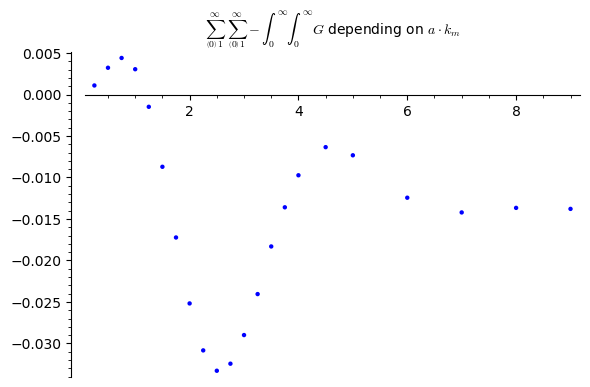
\includegraphics[width=0.46\textwidth]{sum_sum_int_int_G_on_a_km.png}
\caption{}{\centering{\textbf{Рис.2.} Зависимость $\sum\limits_{\left(0\right)\,1}^{\infty}\,\,\sum\limits_{\left(0\right)\,1}^{\infty}-\int\limits_{0}^{\infty}\int\limits_{0}^{\infty}G$ от $a \cdot k_m$.}}
\end{center}
\label{fig:G_on_a_km}
\end{figure}



    Согласно нашему расчёту,

\vspace{-3.5mm}
\begin{equation}
\begin{array}{l}
    \int\limits_{0}^{\infty} \Bigg\{ \sum\limits_{n_x=\left(0\right)\,1}^{\infty} \sum\limits_{n_y=\left(0\right)\,1}^{\infty} F\left(n_x, n_y\right) \\
- \int\limits_{0}^{\infty} \int\limits_{0}^{\infty} F\left(n_x, n_y\right) d{n_x} d{n_y} \Bigg\} d{u} \approx R\left(a k_m\right),
\end{array}
\end{equation}


    где \(R\left(a k_m\right)\) — функция, зависящая от свойств материала, с вполне определённым пределом при \(a\,k_m\,»\,1\). Таким образом,

    \begin{equation}
\delta\,\frac{E}{V} = R\left(a k_m\right)\,\frac{\hbar\,c\,\pi}{a^4}.
\end{equation}

    Для разности плотностей энергии на \(cm^2\) (в пределе \(a\,k_m\,\rightarrow \,10\)) находим

    \(\delta\,\frac{E}{V} = \hbar\,c\, \pi\frac{R}{a^4}\,=\,0.0136\,\frac{1}{a_{\mu}^4}\,dyne/cm^2\)

    где \(a_{\mu}\) — сторона квадратной соты в микронах.


    Можно ли интерпретировать эту разность удельных плотностей энергии \(\delta\left(E/V\right)\) как причину силы \(F\), приложенной к идеально проводящим сотам на пластине? Например, мои исследования конфигурации Казимира показали, что для геометрии двух идеально проводящих пластин \(F/S = -3 \cdot \delta\left(E/V\right)\). А что можно сказать о сотовой конфигурации? Исследование этого вопроса, приведённое в приложениях B и C, показывает, что \(F/S \approx \delta\left(E/V\right)\).

% \end{multicols}

\vspace{\myvspacebeforesubsection}
    \subsection*{\centering{\fontencoding{T2A}\fontfamily{ptm}{\selectfont ЗАКЛЮЧЕНИЕ}}} \label{conclusions}
\vspace{\myvspaceaftersubsection}

% \begin{multicols}{2}

    Таким образом, можно сделать следующие выводы: на идеально проводящие соты на пластине действует сила, обусловленная разностью удельной плотности энергии на её разных сторонах. Эта сила зависит от материала пластины — как минимум от частоты обрезания \(\omega_m\) материала сотовой пластины. Эту силу можно интерпретировать как давление электромагнитных колебаний нулевой точки.

    Хотя эффект мал, экспериментальное подтверждение представляется осуществимым и может представлять определённый интерес.

    Tuo Qu, Fang Liu, Yuechai Lin, Yidong Huang \cite{Tuo2019} сообщили об изготовлении золотых наносот размером около 2 микрон. Согласно формуле, представленной в работе, такие соты должны иметь разность плотностей энергии Казимира около
\(\delta\left(E/V\right) = 0.0136/({2^4}) = 0.0008555\,dyne/cm^2 = 0.0008555 \cdot 10^4 = 8.55\,dyne/m^2\),
т.\,е. 8,55 дин на квадратный метр панели, что является вполне приемлемым значением для практического использования ожидаемого эффекта при коррекции орбит спутников.

    Важно отметить, что в предложенном методе \(\delta\left(E/V\right)\) вычисляется не для полной площади сот, а для части панели, занятой полостями (за вычетом площади стенок сот).

    Это не означает, что стенки сот следует делать как можно тоньше: с уменьшением толщины стенок уменьшается и значение \(k_m\).

    Для простоты расчётов рассмотрены наноячейки квадратной формы, но полученный результат можно использовать — с некоторой пока неизвестной поправкой — для оценки эффекта Казимира в сотах другой формы (шестиугольных, цилиндрических и т.\,д.). Такие соты проще изготовить, но точная оценка эффекта Казимира для них требует гораздо более сложных расчётов. Кроме того, дно соты не обязательно плоское: оно может быть, например, сферически вогнутым, что принципиально не влияет на величину тяги.

    Кроме того, появление тяги Казимира ожидается не только в металлических, но и в диэлектрических сотах, поскольку эффект Казимира в диэлектриках хорошо известен.

    Предполагалось, что высота стенок сот равна \(L/2\), тогда как реальная высота стенок \(h\) будет намного меньше (скажем, порядка \(a\)).

    Вместе с тем, используя подход Антипина (см. приложение D), можно показать, что эффект должен наблюдаться и при меньшей высоте рёбер, хотя зависимость эффекта от высоты может быть предметом дальнейших исследований.

    В ответ Хрвое \cite{Hrvoje2016}, который считает эффект Казимира не следствием существования виртуальных квантовых фотонов, а проявлением дисперсионных сил Лондона–Ван-дер-Ваальса, замечу, что эксперимент по измерению тяги наноячеек, выращенных на металлической пластине, мог бы стать решающим для выяснения того, какая точка зрения на природу силы Казимира соответствует действительности.

\end{multicols}

\vspace{\myvspacebeforesubsection}
    \subsection*{\centering {\fontencoding{T2A}\fontfamily{ptm}{\selectfont \uppercase{Приложение A. Детали интегрирования}}}}\label{appendix-a.-integration-details}
\vspace{\myvspaceaftersubsection}

\begin{multicols}{2}
    Используем регуляризующую функцию в виде

\setcounter{equation}{0}
\renewcommand{\theequation}{A.\arabic{equation}}

\begin{equation}
f\left(\frac{k}{k_m}\right) = \frac{1}{\frac{k^{4}}{k_{m}^{4}} + 1}.
\end{equation}


    Исходя из (\ref{eq:4}) и вводя переменную \(n_{xy} = \sqrt{n_x^2 + n_y^2}\) и \(n = \sqrt{n_x^2 + n_y^2 + u^2} = \sqrt{n_{xy}^2 + u^2}\), имеем 

\noindent
\begin{equation}
F\left(u, n_{xy}, ak_m\right) = \frac{\sqrt{n_{\mathit{xy}}^{2} + u^{2}}}{\frac{\pi^{4} {\left(n_{\mathit{xy}}^{2} + u^{2}\right)}^{2}}{\mathit{ak}_{m}^{4}} + 1}.
\end{equation}


С помощью этой переменной можно сделать следующую подстановку

\vspace{1.5mm}
\(u = \sqrt{n^2 - n_x^2 - n_y^2} = \sqrt{n^2 - n_{xy}^2}\),
\(\frac{du}{dn} = \frac{n}{\sqrt{n^{2} - \mathit{n_{xy}}^{2}}}\), $\,\,\,\,\,\,\,\,\,$
 \(d{u}= \frac{n\,d{n}}{\sqrt{n^{2} - \mathit{n_{xy}}^{2}}}\).

    Теперь интеграл (\ref{eq:5}) можно переписать в виде

\begin{equation}
G%\left(n_x, n_y\right)
 = \int\limits_{0}^{\infty}\sqrt{n_{xy}^2+u^2}\,
f\left(\frac{\pi\sqrt{n_{xy}^2+u^2}}{a\,k_m}\right)\,d{u},
\end{equation}

заменяя переменную интегрирования \(u\) на \(n\)

\noindent
$G%\left(n_x, n_y\right)
 = \int\limits_{n_{xy}}^{\infty}\sqrt{n_{xy}^2+u^2}
 f\left(\frac{\pi\sqrt{n_{xy}^2+u^2}}{a\,k_m}\right)\,dn\,{\frac{n}{\sqrt{n^{2} - n_{xy}^{2}}}}$

\begin{equation}
G\left(n_x, n_y\right) = \int\limits_{n_{xy}}^{\infty}n\,
f\left(\frac{\pi\,n}{a\,k_m}\right)\,dn\,{\frac{n}{\sqrt{n^{2} - n_{xy}^{2}}}},
\end{equation}

    поскольку в таком виде интеграл берётся аналитически. Итак, подынтегральное выражение имеет вид

\begin{equation} \label{eq:A5}
F\left(n, n_{xy}, ak_m\right) = \frac{n^{2}}{{\left(\frac{\pi^{4} n^{4}}{\mathit{ak}_{m}^{4}} + 1\right)} \sqrt{n^{2} - n_{\mathit{xy}}^{2}}}
\end{equation}

    и следующие пределы интегрирования по \(n\): \(n_a = n_{xy}\),
\(n_b = \infty\).

    Используем подстановку Абеля:

\begin{equation}
t = \left(\sqrt{n^2-n_{xy}^2}\right)', \,\,\,\,\,\,\,\,\,\,\, t = \frac{n}{\sqrt{n^{2} - n_{\mathit{xy}}^{2}}}
\end{equation}

    и следующие пределы интегрирования по \(t\): \(t_a = +\infty\),
\(t_b = +1\).

    Обозначим зависимость \(n\) от \(t\)

\begin{equation}
n^{2} = \frac{n_{\mathit{xy}}^{2} t^{2}}{t^{2} - 1}, \,\,\,\,\,\,\,\,\, n = n_{\mathit{xy}} \sqrt{\frac{t^{2}}{t^{2} - 1}}
\end{equation}

    и производные

    \[\frac{dt}{dn} = \frac{d}{dn} \left( \frac{n}{\sqrt{n^{2} - n_{\mathit{xy}}^{2}}} \right)= -\frac{n^{2}}{{\left(n^{2} - n_{\mathit{xy}}^{2}\right)}^{\frac{3}{2}}} + \frac{1}{\sqrt{n^{2} - n_{\mathit{xy}}^{2}}},\]

\begin{equation}
\frac{dn}{dt} = -\frac{n^{4} - 2 \, n^{2} n_{\mathit{xy}}^{2} + n_{\mathit{xy}}^{4}}{\sqrt{n^{2} - n_{\mathit{xy}}^{2}} n_{\mathit{xy}}^{2}}.
\end{equation}

    Теперь перепишем подынтегральное выражение как функцию \(t\)

    \[F\left(t, n_{xy}, ak_m\right) = F\left(n, n_{xy}, ak_m\right) \cdot \frac{dn}{dt} \, \Bigg\rvert_{ n = n_{\mathit{xy}} \sqrt{\frac{t^{2}}{t^{2} - 1}} }\]

\[F\left(n, n_{xy}, ak_m\right) \cdot \frac{dn}{dt} = -\frac{{\left(n^{4} - 2 \, n^{2} n_{\mathit{xy}}^{2} + n_{\mathit{xy}}^{4}\right)} n^{2}}{{\left(\frac{\pi^{4} n^{4}}{\mathit{ak}_{m}^{4}} + 1\right)} {\left(n^{2} - n_{\mathit{xy}}^{2}\right)} n_{\mathit{xy}}^{2}}\]

\[F\left(t, n_{xy}, ak_m\right) = -\frac{{\left(\frac{n_{\mathit{xy}}^{4} t^{4}}{{\left(t^{2} - 1\right)}^{2}} - \frac{2 \, n_{\mathit{xy}}^{4} t^{2}}{t^{2} - 1} + n_{\mathit{xy}}^{4}\right)} t^{2}}{{\left(\frac{\pi^{4} n_{\mathit{xy}}^{4} t^{4}}{{\left(t^{2} - 1\right)}^{2} \mathit{ak}_{m}^{4}} + 1\right)} {\left(\frac{n_{\mathit{xy}}^{2} t^{2}}{t^{2} - 1} - n_{\mathit{xy}}^{2}\right)} {\left(t^{2} - 1\right)}}\]

\[F\left(t, n_{xy}, ak_m\right) = \frac{\mathit{ak}_{m}^{4} n_{\mathit{xy}}^{2} t^{2}}{2 \, \mathit{ak}_{m}^{4} t^{2} - {\left(\pi^{4} n_{\mathit{xy}}^{4} + \mathit{ak}_{m}^{4}\right)} t^{4} - \mathit{ak}_{m}^{4}}\]

    Вынесем из знаменателя коэффициент при \(t^4\).

    Перенесём этот коэффициент в числитель. Новый числитель будет

    \[-\frac{\mathit{ak}_{m}^{4} n_{\mathit{xy}}^{2} t^{2}}{\pi^{4} n_{\mathit{xy}}^{4} + \mathit{ak}_{m}^{4}}.\]

    Соответственно, новый знаменатель будет

    \[-\frac{2 \, \mathit{ak}_{m}^{4} t^{2}}{\pi^{4} n_{\mathit{xy}}^{4} + \mathit{ak}_{m}^{4}} + t^{4} + \frac{\mathit{ak}_{m}^{4}}{\pi^{4} n_{\mathit{xy}}^{4} + \mathit{ak}_{m}^{4}}.\]

    Теперь приведём этот знаменатель к виду

    \[-{\left(\alpha_{1} t + t^{2} + \beta_{1}\right)} {\left(\alpha_{1} t - t^{2} - \beta_{1}\right)},\]

\[t^{4} - {\left(\alpha_{1}^{2} - 2 \, \beta_{1}\right)} t^{2} + \beta_{1}^{2}.\]

    % Begin:

    Итак, имеем уравнение

\[-\frac{2 \, \mathit{ak}_{m}^{4} t^{2}}{\pi^{4} n_{\mathit{xy}}^{4} + \mathit{ak}_{m}^{4}} + t^{4} + \frac{\mathit{ak}_{m}^{4}}{\pi^{4} n_{\mathit{xy}}^{4} + \mathit{ak}_{m}^{4}} = t^{4} - {\left(\alpha_{1}^{2} - 2 \, \beta_{1}\right)} t^{2} + \beta_{1}^{2}\]

и его решение

\begin{equation}\beta_{1} = \frac{\mathit{ak}_{m}^{2}}{\sqrt{\pi^{4} n_{\mathit{xy}}^{4} + \mathit{ak}_{m}^{4}}},\end{equation} \begin{equation}\alpha_{1} = \sqrt{2} \mathit{ak}_{m} \sqrt{\frac{\mathit{ak}_{m}^{2} + \sqrt{\pi^{4} n_{\mathit{xy}}^{4} + \mathit{ak}_{m}^{4}}}{\pi^{4} n_{\mathit{xy}}^{4} + \mathit{ak}_{m}^{4}}}.\end{equation}

    После указанного преобразования подынтегральное выражение можно представить как

    \[\frac{\mathit{ak}_{m}^{4} n_{\mathit{xy}}^{2} t^{2}}{{\left(\pi^{4} n_{\mathit{xy}}^{4} + \mathit{ak}_{m}^{4}\right)} {\left(\alpha_{1} t + t^{2} + \beta_{1}\right)} {\left(\alpha_{1} t - t^{2} - \beta_{1}\right)}}.\]

    Проверим дискриминант \(\alpha_1^2 - 4\beta_1\), используя найденные выше выражения \(\alpha_1\) и \(\beta_1\).

    Дискриминант отрицателен, и интеграл легко вычисляется:

\noindent
    \[\begin{array}{r} \int F\left(t, n_{xy}, ak_m\right) dt = -\frac{\mathit{ak}_{m}^{4} n_{\mathit{xy}}^{2}}{4 \, {\left(\pi^{4} n_{\mathit{xy}}^{4} + \mathit{ak}_{m}^{4}\right)}} \Bigg(\frac{2 \, \arctan\left(\frac{\alpha_{1} + 2 \, t}{\sqrt{-\alpha_{1}^{2} + 4 \, \beta_{1}}}\right)}{\sqrt{-\alpha_{1}^{2} + 4 \, \beta_{1}}} + \\ \frac{2 \, \arctan\left(-\frac{\alpha_{1} - 2 \, t}{\sqrt{-\alpha_{1}^{2} + 4 \, \beta_{1}}}\right)}{\sqrt{-\alpha_{1}^{2} + 4 \, \beta_{1}}} - \frac{\log\left(\alpha_{1} t + t^{2} + \beta_{1}\right)}{\alpha_{1}} + \frac{\log\left(-\alpha_{1} t + t^{2} + \beta_{1}\right)}{\alpha_{1}}\Bigg). \end{array}\]

%    And after substitution of \(t\) value
% \(\int F\left(n, n_{xy}, ak_m\right) dn\) is:

%    \(\begin{array}{r} \int F\left(n, n_{xy}, ak_m\right) dn = -\frac{\mathit{ak}_{m}^{4} n_{\mathit{xy}}^{2}}{4 \, {\left(\pi^{4} n_{\mathit{xy}}^{4} + \mathit{ak}_{m}^{4}\right)}} \Bigg(\frac{2 \, \arctan\left(\frac{\alpha_{1} + \frac{2 \, n}{\sqrt{n^{2} - n_{\mathit{xy}}^{2}}}}{\sqrt{-\alpha_{1}^{2} + 4 \, \beta_{1}}}\right)}{\sqrt{-\alpha_{1}^{2} + 4 \, \beta_{1}}} + \\ \frac{2 \, \arctan\left(-\frac{\alpha_{1} - \frac{2 \, n}{\sqrt{n^{2} - n_{\mathit{xy}}^{2}}}}{\sqrt{-\alpha_{1}^{2} + 4 \, \beta_{1}}}\right)}{\sqrt{-\alpha_{1}^{2} + 4 \, \beta_{1}}} - \frac{\log\left(\frac{\alpha_{1} n}{\sqrt{n^{2} - n_{\mathit{xy}}^{2}}} + \beta_{1} + \frac{n^{2}}{n^{2} - n_{\mathit{xy}}^{2}}\right)}{\alpha_{1}} + \frac{\log\left(-\frac{\alpha_{1} n}{\sqrt{n^{2} - n_{\mathit{xy}}^{2}}} + \beta_{1} + \frac{n^{2}}{n^{2} - n_{\mathit{xy}}^{2}}\right)}{\alpha_{1}}\Bigg) \end{array}\)

%    Checking that found integral is true by differentiation:

%     \[\left( \int F\left(n, n_{xy}, ak_m\right) dn \right)' = \frac{\sqrt{n^{2} - n_{\mathit{xy}}^{2}} \mathit{ak}_{m}^{4} n^{2}}{\pi^{4} n^{6} + \mathit{ak}_{m}^{4} n^{2} - {\left(\pi^{4} n^{4} + %  % \mathit{ak}_{m}^{4}\right)} n_{\mathit{xy}}^{2}}\]

% \[F\left(n, n_{xy}, ak_m\right)= \frac{n^{2}}{{\left(\frac{\pi^{4} n^{4}}{\mathit{ak}_{m}^{4}} + 1\right)} \sqrt{n^{2} - n_{\mathit{xy}}^{2}}}\]

% \[\left( \int F\left(n, n_{xy}, ak_m\right) dn \right)'-F\left(n, n_{xy}, ak_m\right) = 0\]

%    So, we received true expression of integral
% \(\int F\left(n, n_{xy}, ak_m\right) dn\)

% Now using its \(t_a\) and \(t_b\) limits we found the following
% integral:

    % \(\begin{array}{r}  G\left(n_{xy}\right) = \int\limits_{0}^{\infty}\sqrt{n_{xy}^2+u^2}\, f\left(\frac{\pi\sqrt{n_{xy}^2+u^2}}{a\,k_m}\right)\,d{u} = \\  -\frac{\mathit{ak}_{m}^{4} n_{\mathit{xy}}^{2} {\left(\frac{2 \, \arctan\left(\frac{\alpha_{1} + 2}{\sqrt{-\alpha_{1}^{2} + 4 \, \beta_{1}}}\right)}{\sqrt{-\alpha_{1}^{2} + 4 \, \beta_{1}}} + \frac{2 \, \arctan\left(-\frac{\alpha_{1} - 2}{\sqrt{-\alpha_{1}^{2} + 4 \, \beta_{1}}}\right)}{\sqrt{-\alpha_{1}^{2} + 4 \, \beta_{1}}} - \frac{\log\left(\alpha_{1} + \beta_{1} + 1\right)}{\alpha_{1}} + \frac{\log\left(-\alpha_{1} + \beta_{1} + 1\right)}{\alpha_{1}}\right)}}{4 \, {\left(\pi^{4} n_{\mathit{xy}}^{4} + \mathit{ak}_{m}^{4}\right)}} \\ +\frac{\pi \mathit{ak}_{m}^{4} n_{\mathit{xy}}^{2}}{2 \, {\left(\pi^{4} \sqrt{-\alpha_{1}^{2} + 4 \, \beta_{1}} n_{\mathit{xy}}^{4} + \sqrt{-\alpha_{1}^{2} + 4 \, \beta_{1}} \mathit{ak}_{m}^{4}\right)}} \end{array}\)


\end{multicols}

\pagebreak

\vspace{\myvspacebeforesubsection}
    \subsection*{\centering {\fontencoding{T2A}\fontfamily{ptm}{\selectfont \uppercase{Приложение B. Расчёт электромагнитного давления}}}} \label{appendix-b.-electromagnetic-pressure-calculation}
\vspace{\myvspaceaftersubsection}

\begin{multicols}{2}

\setcounter{equation}{0}
\renewcommand{\theequation}{B.\arabic{equation}}

    Рассмотрим прямоугольный резонатор размером \(a \times b \times h\).

    \textbf{Для электрической моды}

\begin{equation}\nabla\,\vec{E} + \frac{\omega^2}{c^2}\,\vec{E} = 0,\end{equation} имеем следующее решение

\[E_{x} = A_{x} \cos\left(\frac{\pi n_{x} x}{a}\right) \sin\left(\frac{\pi n_{y} y}{b}\right) \sin\left(k_{z} z\right)\]
\[E_{y} = A_{y} \cos\left(\frac{\pi n_{y} y}{b}\right) \sin\left(\frac{\pi n_{x} x}{a}\right) \sin\left(k_{z} z\right)\]
\[E_{z} = A_{z} \cos\left(k_{z} z\right) \sin\left(\frac{\pi n_{x} x}{a}\right) \sin\left(\frac{\pi n_{y} y}{b}\right)\]

и
\[H_{x} = \frac{i \, {\left(A_{y} b k_{z} - \pi A_{z} n_{y}\right)} c \cos\left(\frac{\pi n_{y} y}{b}\right) \cos\left(k_{z} z\right) \sin\left(\frac{\pi n_{x} x}{a}\right)}{b \mu \omega}\]
\[H_{y} = -\frac{i \, {\left(A_{x} k_{z} - \frac{\pi A_{z} n_{x}}{a}\right)} c \cos\left(\frac{\pi n_{x} x}{a}\right) \cos\left(k_{z} z\right) \sin\left(\frac{\pi n_{y} y}{b}\right)}{\mu \omega}\]
\[H_{z} = -\frac{i \, {\left(\frac{\pi A_{y} n_{x}}{a} - \frac{\pi A_{x} n_{y}}{b}\right)} c \cos\left(\frac{\pi n_{x} x}{a}\right) \cos\left(\frac{\pi n_{y} y}{b}\right) \sin\left(k_{z} z\right)}{\mu \omega}\]

при
\begin{equation}k_{z}^{2} + \frac{\pi^{2} n_{x}^{2}}{a^{2}} + \frac{\pi^{2} n_{y}^{2}}{b^{2}} - \frac{\omega^{2}}{c^{2}} = 0,\end{equation}

используя \(div\,\vec{E} = 0\), получаем

\begin{equation}A_{z} k_{z} + \frac{\pi A_{x} n_{x}}{a} + \frac{\pi A_{y} n_{y}}{b} = 0.\end{equation}

Плотность энергии поля
\(\left(\int \frac{E_x^2+E_y^2+E_z^2}{8 \pi}dV\right)\big/{V}\) равна

\begin{equation}\frac{E}{V} = \frac{{A_{x}^{2} + A_{y}^{2} + A_{z}^{2}} }{64 \, \pi}.\end{equation}

    Полная плотность энергии
% \(\left(\int \frac{E_x^2+E_y^2+E_z^2}{8 \pi}dV + \int \frac{H_x^2+H_y^2+H_z^2}{8 \pi}dV\right)\big/{V}\)
\(\left(\int \frac{|\vec{E}|^2}{8 \pi}dV + \int \frac{|\vec{H}|^2}{8 \pi}dV\right)\big/{V}\) равна

\begin{equation}\frac{E}{V} = \frac{{A_{x}^{2} + A_{y}^{2} + A_{z}^{2}}}{32 \, \pi}.\end{equation}

    Электромагнитное давление
\(\left({\int \frac {H_x^2+H_y^2}{8 \pi} dS}\right)\big/{S}\) на пластину \(xy\) равно

\end{multicols}

% \renewcommand{\theequation}{B.\arabic{equation}}

\begin{equation}\frac{f_z}{S} = -\frac{2 \, \pi A_{x} A_{z} a b^{2} k_{z} n_{x} - \pi^{2} A_{z}^{2} b^{2} n_{x}^{2} + 2 \, \pi A_{y} A_{z} a^{2} b k_{z} n_{y} - \pi^{2} A_{z}^{2} a^{2} n_{y}^{2} - {\left(A_{x}^{2} + A_{y}^{2}\right)} a^{2} b^{2} k_{z}^{2}}{32 \, {\left(\pi a^{2} b^{2} k_{z}^{2} + \pi^{3} b^{2} n_{x}^{2} + \pi^{3} a^{2} n_{y}^{2}\right)}}.\end{equation}

    Их отношение \(\frac{f_z/S}{E/V}\) равно

\begin{equation}\frac{f_z/S}{E/V} = \frac{A_{x}^{2} a^{2} b^{2} k_{z}^{2} + A_{y}^{2} a^{2} b^{2} k_{z}^{2} - 2 \, \pi A_{x} A_{z} a b^{2} k_{z} n_{x} + \pi^{2} A_{z}^{2} b^{2} n_{x}^{2} - 2 \, \pi A_{y} A_{z} a^{2} b k_{z} n_{y} + \pi^{2} A_{z}^{2} a^{2} n_{y}^{2}}{{\left(a^{2} b^{2} k_{z}^{2} + \pi^{2} b^{2} n_{x}^{2} + \pi^{2} a^{2} n_{y}^{2}\right)} {\left(A_{x}^{2} + A_{y}^{2} + A_{z}^{2}\right)}}.\end{equation}

\begin{multicols}{2}

    Рассматривая решение с распространением волны вдоль \(z\) имеем
\(H_z = 0\) что даёт

    \[\pi A_{y} b n_{x} - \pi A_{x} a n_{y} = 0\]

    и
\[A_{x} = -\frac{A_{z} a b^{2} k_{z} n_{x}}{\pi b^{2} n_{x}^{2} + \pi a^{2} n_{y}^{2}},
A_{y} = -\frac{A_{z} a^{2} b k_{z} n_{y}}{\pi b^{2} n_{x}^{2} + \pi a^{2} n_{y}^{2}}.\]

    В этом случае отношение электромагнитного давления к плотности энергии поля равно \(1\),

\begin{equation}\frac{f_z/S}{E/V} = 1.\end{equation}

    Рассматривая решение с распространением волны вдоль \(x\) имеем
\(H_x = 0\) что даёт

    \[A_{y} = -\frac{\pi^{2} A_{x} b n_{x} n_{y}}{a b^{2} k_{z}^{2} + \pi^{2} a n_{y}^{2}},
A_{z} = -\frac{\pi A_{x} b^{2} k_{z} n_{x}}{a b^{2} k_{z}^{2} + \pi^{2} a n_{y}^{2}}.\]

    В этом случае отношение электромагнитного давления к плотности энергии поля равно

\begin{equation}\frac{f_z/S}{E/V} = \frac{b^{2} k_{z}^{2}}{b^{2} k_{z}^{2} + \pi^{2} n_{y}^{2}}.\end{equation}

    Рассматривая решение с распространением волны вдоль \(y\),
\(H_y = 0\), как и для \(x\)

\[A_{x} = -\frac{\pi^{2} A_{y} a n_{x} n_{y}}{a^{2} b k_{z}^{2} + \pi^{2} b n_{x}^{2}},
A_{z} = -\frac{\pi A_{y} a^{2} k_{z} n_{y}}{a^{2} b k_{z}^{2} + \pi^{2} b n_{x}^{2}},\]

\begin{equation}\frac{f_z/S}{E/V} = \frac{a^{2} k_{z}^{2}}{a^{2} k_{z}^{2} + \pi^{2} n_{x}^{2}}.\end{equation}

    \textbf{Для магнитной моды}

\begin{equation}\nabla\,\vec{H} + \frac{\omega^2}{c^2}\,\vec{H} = 0\end{equation}, имеем следующее решение

    \[H_{x} = B_{1} \cos\left(\frac{\pi n_{y} y}{b}\right) \cos\left(k_{z} z\right) \sin\left(\frac{\pi n_{x} x}{a}\right)\]
\[H_{y} = B_{2} \cos\left(\frac{\pi n_{x} x}{a}\right) \cos\left(k_{z} z\right) \sin\left(\frac{\pi n_{y} y}{b}\right)\]
\[H_{z} = B_{3} \cos\left(\frac{\pi n_{x} x}{a}\right) \cos\left(\frac{\pi n_{y} y}{b}\right) \sin\left(k_{z} z\right)\]

    и
\[E_{x} = \frac{i \, {\left(B_{2} k_{z} - \frac{\pi B_{3} n_{y}}{b}\right)} c \cos\left(\frac{\pi n_{x} x}{a}\right) \sin\left(\frac{\pi n_{y} y}{b}\right) \sin\left(k_{z} z\right)}{\mu \omega}\]
\[E_{y} = -\frac{i \, {\left(B_{1} k_{z} - \frac{\pi B_{3} n_{x}}{a}\right)} c \cos\left(\frac{\pi n_{y} y}{b}\right) \sin\left(\frac{\pi n_{x} x}{a}\right) \sin\left(k_{z} z\right)}{\mu \omega}\]
\[E_{z} = -\frac{i \, {\left(\frac{\pi B_{2} n_{x}}{a} - \frac{\pi B_{1} n_{y}}{b}\right)} c \cos\left(k_{z} z\right) \sin\left(\frac{\pi n_{x} x}{a}\right) \sin\left(\frac{\pi n_{y} y}{b}\right)}{\mu \omega}\]

    при
\begin{equation}k_{z}^{2} + \frac{\pi^{2} n_{x}^{2}}{a^{2}} + \frac{\pi^{2} n_{y}^{2}}{b^{2}} - \frac{\omega^{2}}{c^{2}} = 0,\end{equation}

    используя \(div\,\vec{H} = 0\), получаем

\begin{equation}B_{3} k_{z} + \frac{\pi B_{1} n_{x}}{a} + \frac{\pi B_{2} n_{y}}{b} = 0.\end{equation}

    Плотность энергии магнитного поля
\(\left(\int \frac{H_x^2+H_y^2+H_z^2}{8 \pi}dV\right)\big/{V}\) равна

\begin{equation}\frac{E}{V} = \frac{{B_{1}^{2} + B_{2}^{2} + B_{3}^{2}}}{64 \, \pi}.\end{equation}

    Полная плотность энергии
\(\left(\int \frac{|\vec{E}|^2}{8 \pi}dV + \int \frac{|\vec{H}|^2}{8 \pi}dV\right)\big/{V}\) равна

\begin{equation}\frac{E}{V} = \frac{{B_{1}^{2} + B_{2}^{2} + B_{3}^{2}}}{32 \, \pi}.\end{equation}

    Электромагнитное давление
\(\left({\int \frac {H_x^2+H_y^2}{8 \pi} dS}\right)\big/{S}\) на пластину \(xy\) равно

\begin{equation}\frac{f_z}{S}=\frac{{B_{1}^{2} + B_{2}^{2}}}{32 \, \pi}.\end{equation}

Их отношение \(\frac{f_z/S}{E/V}\) равно

\begin{equation}\frac{f_z/S}{E/V} = \frac{{B_{1}^{2} + B_{2}^{2}}}{B_{1}^{2} + B_{2}^{2} + B_{3}^{2}}.\end{equation}

Рассматривая решение с распространением волны вдоль \(z\), имеем
\(E_z = 0\) что даёт

\[\frac{\pi B_{2} n_{x}}{a} - \frac{\pi B_{1} n_{y}}{a} = 0\]

и
\[B_1 = -\frac{B_{3} a k_{z} n_{x}}{\pi n_{x}^{2} + \pi n_{y}^{2}},
B_2 = -\frac{B_{3} a k_{z} n_{y}}{\pi n_{x}^{2} + \pi n_{y}^{2}}.\]

В этом случае отношение электромагнитного давления к плотности энергии поля равно

\begin{equation}\frac{f_z/S}{E/V} = \frac{a^{2} k_{z}^{2}}{a^{2} k_{z}^{2} + \pi^{2} n_{x}^{2} + \pi^{2} n_{y}^{2}}.\end{equation}

    Рассматривая решение с распространением волны вдоль \(x\), имеем
\(E_x = 0\) что даёт

\[B_2 = -\frac{\pi^{2} B_{1} n_{x} n_{y}}{a^{2} k_{z}^{2} + \pi^{2} n_{y}^{2}},
B_3 = -\frac{\pi B_{1} a k_{z} n_{x}}{a^{2} k_{z}^{2} + \pi^{2} n_{y}^{2}}.\]

В этом случае отношение электромагнитного давления к плотности энергии поля равно

\[\frac{f_z/S}{E/V} = \frac{a^{2} b^{4} k_{z}^{4} + 2 \, \pi^{2} a^{2} b^{2} k_{z}^{2} n_{y}^{2} + \pi^{4} b^{2} n_{x}^{2} n_{y}^{2} + \pi^{4} a^{2} n_{y}^{4}}{{\left(a^{2} b^{2} k_{z}^{2} + \pi^{2} b^{2} n_{x}^{2} + \pi^{2} a^{2} n_{y}^{2}\right)} {\left(b^{2} k_{z}^{2} + \pi^{2} n_{y}^{2}\right)}}.\]

Рассматривая решение с распространением волны вдоль \(y\)
\(E_y = 0\) как и для \(x\)

    \[B_1 = -\frac{\pi^{2} B_{2} n_{x} n_{y}}{a^{2} k_{z}^{2} + \pi^{2} n_{x}^{2}},
      B_3 = -\frac{\pi B_{2} a k_{z} n_{y}}{a^{2} k_{z}^{2} + \pi^{2} n_{x}^{2}},\]

\[\frac{f_z/S}{E/V} = \frac{a^{4} b^{2} k_{z}^{4} + 2 \, \pi^{2} a^{2} b^{2} k_{z}^{2} n_{x}^{2} + \pi^{4} b^{2} n_{x}^{4} + \pi^{4} a^{2} n_{x}^{2} n_{y}^{2}}{{\left(a^{2} b^{2} k_{z}^{2} + \pi^{2} b^{2} n_{x}^{2} + \pi^{2} a^{2} n_{y}^{2}\right)} {\left(a^{2} k_{z}^{2} + \pi^{2} n_{x}^{2}\right)}}.\]

    Итак, задача расчёта электромагнитной силы в конфигурации наносот оказывается достаточно простой, поскольку

\begin{equation}\lim_{k_z \to \infty}\frac{f_z/S}{E/V} = 1.\end{equation}

Видно, что при уменьшении \(a\) отношение \(\frac{f_z/S}{E/V}\) также уменьшается, что приводит к

\begin{equation}\frac{F}{S} \geq \delta\,\frac{E}{V} = \hbar\,c\, \pi\frac{R}{a^4}.\end{equation}

С другой стороны, тот же результат можно показать с помощью гамильтоновой механики.

% \end{multicols}

\vspace{\myvspacebeforesubsection}
    \subsection*{\centering {\fontencoding{T2A}\fontfamily{ptm}{\selectfont \uppercase{Приложение C. Подход гамильтоновой механики}}}} \label{appendix-c.-hamiltonian-mechanics-approach}
\vspace{\myvspaceaftersubsection}

% \begin{multicols}{2}

\setcounter{equation}{0}
\renewcommand{\theequation}{C.\arabic{equation}}

    Рассмотрим кубический резонатор объёмом \(L^3\), ограниченный идеально
проводящими стенками, в который помещена идеально проводящая квадратная пластина со стороной
\(L\), параллельная грани \(xy\), причём расстояние между пластиной и гранью \(xy\) достаточно велико, например \(l = L/2\).

Одна сторона этой идеально проводящей квадратной пластины — гладкая плоскость, а
другая покрыта идеально проводящими сотами квадратной формы со стороной квадрата \(a\).

По обе стороны пластины выражения \(1\big/2\sum\,\hbar\omega\)
где суммирование ведётся по всем возможным резонансным частотам резонатора \(\left(L-l\right)\times L\times L\) (большой резонатор между гладкой плоскостью и гранью \(xy\)) and the cavity \(l\times a\times a\) (малый резонатор — одна ячейка сот) расходятся и лишены физического смысла, однако будет показано, что для обеих противоположных сторон производная \({d\left<0|\hat{\mathcal{H}}|0\right>}\big/{dl}\) вакуумного гамильтониана всей системы для этих сумм
\(\left<0|\hat{\mathcal{H}}|0\right> = 1\big/2\,\left(\sum\,\,\hbar\omega\right)_{I} + 1\big/2\,\left(\sum\,\,\hbar\omega\right)_{II}\),
имеет вполне определённое значение, и это значение будет интерпретировано как взаимодействие между пластиной и обеими гранями \(xy\).

\begin{figure}
\begin{center}
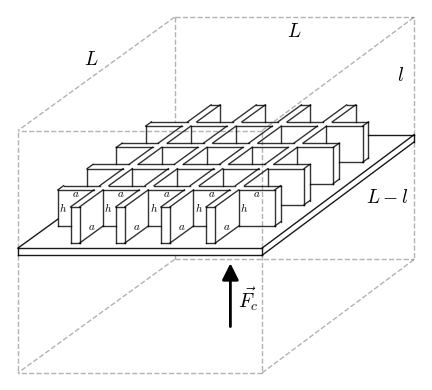
\includegraphics[width=0.42\textwidth]{honeycomb_box_H.png}
\caption{}{\centering{\textbf{Рис.3.} Кубический резонатор с пластиной, покрытой сотами.}}
\end{center}
\label{fig:honeycomb_box_H}
\end{figure}

    Возможные колебания резонаторов, задаваемых условиями
\(0 \leq x \leq L\), \(0 \leq y \leq L\), \(0 \geq z \geq -\,(L-l)\) (большой резонатор между гладкой плоскостью и гранью \(xy\))
и
\(0 \leq x \leq a\), \(0 \leq y \leq a\), \(0 \leq z \leq l\) (малый резонатор — одна ячейка сот)
    имеют волновые векторы
\(k_x = \frac{\pi}{L}\,n_x\), \(k_y = \frac{\pi}{L}\,n_y\),
\(k_z = \frac{\pi}{L-l}\,n_z\) (большой резонатор между гладкой плоскостью и гранью \(xy\)),
и
\(k_x = \frac{\pi}{a}\,n_x\), \(k_y = \frac{\pi}{a}\,n_y\),
\(k_z = \frac{\pi}{l}\,n_z\) (малый резонатор — одна ячейка сот),
где \(n_x\), \(n_y\), \(n_z\) — целые положительные числа;
\(k = \sqrt{k_x^2+k_y^2+k_z^2} = \sqrt{\kappa^2+k_z^2}\).

Запишем выражение для суммы энергии нулевых колебаний в общем виде

\begin{equation}
E = \frac{1}{2}\sum\,\hbar\omega = \hbar\,c\frac{1}{2}\sum\limits_{n_x}^{}\sum\limits_{n_y}^{}\sum\limits_{n_z}^{}k.
\end{equation}

    Каждому набору \(k_x\), \(k_y\), \(k_z\) соответствуют две стоячие волны, но если одно из \(n_i\) равно нулю, волна только одна. Для резонатора одной ячейки сот это несущественно по \(k_z\), поскольку при очень большом \(l\) можно считать \(k_z\) непрерывной переменной, заменив суммирование по \(n_z\) интегрированием.
Таким образом, для малого резонатора из одной соты находим

\noindent
\(E = \frac{\hbar c}{2}\int\limits_{0}^{\infty}\left[{\sqrt{k_z^2}+2\sum\limits_{n_x=1}^{\infty}\sum\limits_{n_y=1}^{\infty}\sqrt{\frac{n_x^2\pi^2}{a^2}+\frac{n_y^2\pi^2}{a^2}+k_z^2}}\right]d{n_z}\).

    Учитывая \(dn_z = \frac{l}{\pi}\,dk_z\) можно найти удельную плотность энергии \(E/S\), где
\(S = S_{small} = a^2\):

\noindent
    \(\frac{E}{S} = \frac{\hbar c}{a^2}\int\limits_{0}^{\infty}\left[{\frac{\sqrt{k_z^2}}{2}+\sum\limits_{n_x=1}^{\infty}\sum\limits_{n_y=1}^{\infty}\sqrt{\frac{n_x^2\pi^2}{a^2}+\frac{n_y^2\pi^2}{a^2}+k_z^2}}\right]\frac{l}{\pi}dk_z\),

\noindent
    \(\frac{E}{S} = \frac{\hbar c l}{a^2 \pi} \sum\limits_{n_x=(0)1}^{\infty}
\sum\limits_{n_y=(0)1}^{\infty}\Bigg[\int\limits_{0}^{\infty}\sqrt{\frac{n_x^2\pi^2}{a^2}+\frac{n_y^2\pi^2}{a^2}+k_z^2}\,dk_z\Bigg]\).

    Для большого резонатора это несущественно по \(k_x\), \(k_y\), поскольку при очень большом \(L\) можно считать \(k_x\), \(k_y\) непрерывными переменными. Таким образом, для большого резонатора между гладкой плоскостью и гранью \(xy\) находим
\noindent
\begin{equation}\begin{array}{l}
\begin{array}{ll}
\sum\frac{\hbar\omega}{2} = \frac{\hbar c}{2}\int\limits_{0}^{\infty}\int\limits_{0}^{\infty}\Bigg[\sqrt{k_x^2+k_y^2}\,+ & \,\\
\end{array} \\
\begin{array}{rr}
\,\,\,\,\,\,\,\,\,\,\,+ & 2\sum\limits_{n_z=1}^{\infty}\sqrt{\frac{n_z^2 \pi^2}{(L-l)^2}+k_x^2+k_y^2}\Bigg]d{n_x}d{n_y}.\end{array}
\end{array}\end{equation}

%\(\sum\frac{\hbar\omega}{2} = \frac{\hbar c}{2}\int\limits_{0}^{\infty}\int\limits_{0}^{\infty}\left[{\sqrt{k_x^2+k_y^2}+ \\
%2\sum\limits_{n_z=1}^{\infty}\sqrt{\frac{n_z^2 \pi^2}{(L-l)^2}+k_x^2+k_y^2}}\right]d{n_x}d{n_y}\)
% (large cavity between pure plane and \(xy\) face),

При очень большом \(L-l\) последнее суммирование можно заменить интегралом; следовательно, энергия большого резонатора равна
\noindent
\begin{equation}\sum\frac{\hbar\omega}{2} = \hbar\,c\int\limits_{0}^{\infty}\int\limits_{0}^{\infty}\int\limits_{0}^{\infty}\sqrt{k_z^2+k_x^2+k_y^2}\,d{n_x}\,d{n_y}\,d{n_z},\end{equation}
% (large cavity between pure plane and \(xy\) face),

где \(dn_x = \frac{L}{\pi}\,dk_x\), \(dn_y = \frac{L}{\pi}\,dk_y\),
\(dn_z = \frac{L-l}{\pi}\,dk_z\).

    Теперь для удельной (на единицу площади) плотности энергии \(E/S\) большого резонатора, где
\(S = S_{large} = L^2\) можно записать следующую цепочку преобразований:

\noindent
\(\frac{\sum\hbar\omega}{2 S} = \frac{\hbar\,c}{L^2}\int\limits_{0}^{\infty}\int\limits_{0}^{\infty}\int\limits_{0}^{\infty}\sqrt{k_z^2+k_x^2+k_y^2}\,dn_x\,dn_y\,\frac{L-l}{\pi}\,dk_z\),
% (large cavity between pure plane and \(xy\) face),

%\noindent
%\(\frac{\sum\hbar\omega}{2 S} = \frac{L-l}{L^2\,\pi}\hbar\,c\int\limits_{0}^{\infty}\int\limits_{0}^{\infty}\left[\,\int\limits_{0}^{\infty}\sqrt{k_z^2+k_x^2+k_y^2}\,dk_z\right]\,dn_x\,dn_y\),
% (large cavity between pure plane and \(xy\) face),

\noindent
\(\frac{E}{S} = \frac{L-l}{L^2\,\pi}\hbar\,c\int\limits_{0}^{\infty}\int\limits_{0}^{\infty}\left[\,\int\limits_{0}^{\infty}\sqrt{k_x^2+k_y^2+k_z^2}\,dk_z\right] \left(\frac{L}{\pi}dk_x\right) \left(\frac{L}{\pi}dk_y\right)\),
% (large cavity between pure plane and \(xy\) face),

\noindent
\(\frac{E}{S} = \frac{L-l}{a^2\,\pi}\hbar\,c\int\limits_{0}^{\infty}\int\limits_{0}^{\infty}\left[\,\int\limits_{0}^{\infty}\sqrt{k_x^2+k_y^2+k_z^2}\,dk_z\right] \left(\frac{a}{\pi}dk_x\right) \left(\frac{a}{\pi}dk_y\right)\).
% (large cavity between pure plane and \(xy\) face).

    Отсюда видно, что удельный (на единицу площади) вакуумный гамильтониан
\(\frac{\left<0|\hat{\mathcal{H}}|0\right>}{S}\) всей системы равен

\end{multicols}

% \noindent
% \[\begin{array}{lr}
% % \frac{\left<0|\hat{\mathcal{H}}|0\right>}{S} =
% \begin{array}{l}
% \frac{\left<0|\hat{\mathcal{H}}|0\right>}{S} = \frac{\hbar\,c}{a^2\,\pi} \cdot\\
% \cdot \Bigg\{l\sum\limits_{n_x=(0)1}^{\infty}\sum\limits_{n_y=(0)1}^{\infty}%\left[\,\int\limits_{0}^{\infty}\sqrt{n_x^2\frac{\pi^2}{a^2}+n_y^2\frac{\pi^2}{a^2}+k_z^2}\,dk_z\right] + \\
% (L-l)\int\limits_{0}^{\infty}\int\limits_{0}^{\infty}\left[\,\int\limits_{0}^{\infty}\sqrt{k_x^2+k_y^2+k_z^2}\,dk_z\right]\,\left(\frac{a}{\pi}dk_x\right)\,\left(\frac{a}{\pi}dk_y\right)\Bigg\}
% \end{array}\end{array}\]

\noindent
\[
\frac{\left<0|\hat{\mathcal{H}}|0\right>}{S} = \frac{\hbar\,c}{a^2\,\pi}
\cdot \Bigg\{l\sum\limits_{n_x=(0)1}^{\infty}\sum\limits_{n_y=(0)1}^{\infty}\left[\,\int\limits_{0}^{\infty}\sqrt{n_x^2\frac{\pi^2}{a^2}+n_y^2\frac{\pi^2}{a^2}+k_z^2}\,dk_z\right] +
(L-l)\int\limits_{0}^{\infty}\int\limits_{0}^{\infty}\left[\,\int\limits_{0}^{\infty}\sqrt{k_x^2+k_y^2+k_z^2}\,dk_z\right]\,\left(\frac{a}{\pi}dk_x\right)\,\left(\frac{a}{\pi}dk_y\right)\Bigg\}
\]

и взаимодействие
\(\frac{F}{S} = -\frac{\partial }{\partial z} \,\frac{\left<0|\hat{\mathcal{H}}|0\right>}{S} = \frac{\partial}{\partial l} \,\frac{\left<0|\hat{\mathcal{H}}|0\right>}{S}\) равно

%\(\begin{array}{lr}\frac{F}{S} =
%\begin{array}{c}\frac{\hbar\,c}{a^2\,\pi}\Bigg\{\sum\limits_{n_x=(0)1}^{\infty}\sum\limits_{n_y=(0)1}^{\infty}\left[\,\int\limits_{0}^{\infty}\sqrt{n_x^2\frac{\pi^2}{a^2}+n_y^2\frac{\pi^2}{a^2}+k_z^2}\,dk_z\right] - \\
%\int\limits_{0}^{\infty}\int\limits_{0}^{\infty}\left[\,\int\limits_{0}^{\infty}\sqrt{k_x^2+k_y^2+k_z^2}\,dk_z\right]\,dn_x\,dn_y\Bigg\}\end{array}\end{array}\)

\noindent
\begin{equation}\frac{F}{S} = \frac{\hbar\,c}{a^2\,\pi}\left\{\sum\limits_{n_x=(0)1}^{\infty}\sum\limits_{n_y=(0)1}^{\infty}\left[\,\int\limits_{0}^{\infty}\sqrt{n_x^2\frac{\pi^2}{a^2}+n_y^2\frac{\pi^2}{a^2}+k_z^2}\,dk_z\right] -
\int\limits_{0}^{\infty}\int\limits_{0}^{\infty}\left[\,\int\limits_{0}^{\infty}\sqrt{k_x^2+k_y^2+k_z^2}\,dk_z\right]\,dn_x\,dn_y\right\}\end{equation}

\begin{multicols}{2}

    Таким образом, формула для силы \({F}/{S}\), действующей на идеально проводящие соты на пластине, полученная методами гамильтоновой механики, совпадает с формулой (\ref{eq:2}), полученной для разности удельных плотностей энергии на её разных сторонах \(\delta\left({E}/{V}\right)\).

%    \begin{wrapfigure}{r}{0.5\textwidth}
%\begin{center}
%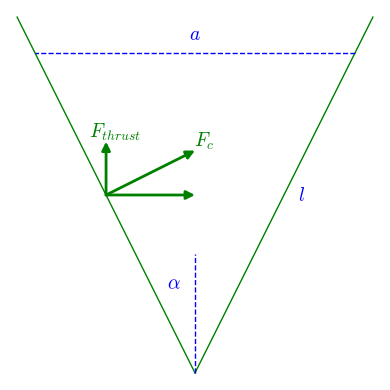
\includegraphics[width=0.48\textwidth]{Antipins_angle_en.png}
%\caption{}{Antipin's angle}
%\end{center}
%\label{fig:Antipins_angle}
%\end{wrapfigure}



\end{multicols}
\begin{multicols}{2}

\vspace{\myvspacebeforesubsection}
    \subsection*{\centering {\fontencoding{T2A}\fontfamily{ptm}{\selectfont \uppercase{Приложение D. Вывод формулы тяги для сот на основе формулы Антипина для металлического уголка}}}} \label{appendix-d.-the-derivation-of-the-thrust-formula-for-the-honeycomb-basing-on-the-antipin-formula-for-the-thrust-of-a-metal-angle}
\vspace{\myvspaceaftersubsection}

\setcounter{equation}{0}
\renewcommand{\theequation}{D.\arabic{equation}}

    Антипин \cite{Antipin2012} даёт оценочный расчёт тяги \mbox{V-образного} уголка с помощью формулы Казимира «в наиболее общих и естественных приближениях, известных как метод PFA (Proximity Force Approximation) или PAA (Pairwise Additive Approximation) \cite{Intravaia2013}, \cite{Rodriguez2011}».

\begin{figure}
\begin{center}
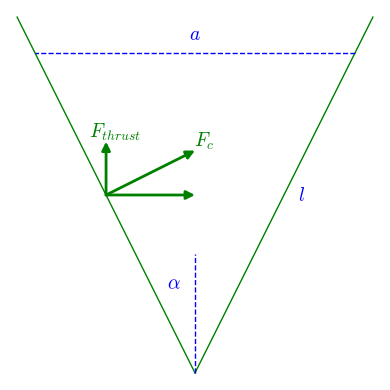
\includegraphics[width=0.45\textwidth]{Antipins_angle_en.png}
\caption{}{\centering{\textbf{Рис.4.} Уголок Антипина.}}
\end{center}
\label{fig:Antipins_angle}
\end{figure}


Энергия взаимодействия Казимира равна
\noindent
\begin{equation}\delta\,E/L^2 = \hbar\,c\frac{\pi^2}{4\,a^3}\left\{\frac{-4}{24\times30}\right\}.\end{equation}

Сила Казимира равна
\noindent
\begin{equation}F_{c} = \hbar\,c\frac{-3\,\pi^2}{4\,a^4}\left\{\frac{-4}{24\times30}\right\}.\end{equation}

Тяга металлического \mbox{V-образного} уголка равна
\noindent
\begin{equation}F_{thrust} = 2 \int F_{c} \, sin\, \alpha \,dS, \,\,\,\,\,\,\, dS = b\,dz\end{equation}

\noindent
\begin{equation}F_{thrust} = 2\, \frac{-3\,\pi^2\hbar c b}{4}\int\limits_{z_{min}}^{z_{max}} \left\{\frac{-4}{24\times30}\right\}\frac{sin\, \alpha\,dz}{\left(a\left(z\right)\right)^4}.\end{equation}

Сделаем подстановку

\[a\left(z\right) = 2\,z\,tg\, \alpha,\]

\[F_{thrust} = 2\, \frac{-3\,\pi^2\hbar c b}{4}\int\limits_{z_{min}}^{z_{max}} \left\{\frac{-4}{24\times30}\right\}\frac{sin\, \alpha\,dz}{\left(2\,z\,tg \alpha\right)^4},\]

\[F_{thrust} = 2\, \frac{-3\,\pi^2\hbar c b}{4} \frac{sin\, \alpha}{\left(2\,tg\, \alpha\right)^4} \int\limits_{z_{min}}^{z_{max}} \left\{\frac{-4}{24\times30}\right\} \frac{dz}{z^4},\]

\[F_{thrust} = -2\cdot3\, \frac{\pi^2\hbar c b}{240} \frac{sin\, \alpha}{\left(2\,tg\, \alpha\right)^4} \left(\frac{1}{z^3}\right)\Bigg\rvert_{\,z_{min}.}^{\,z_{max}} \]

    Можно сделать следующую подстановку: \[z = l\, cos\, \alpha,\]

\[F_{thrust} = -2\cdot3\, \frac{\pi^2\hbar c b}{240} \frac{sin\, \alpha}{2^4\left(tg\,\alpha\right)^4\left(cos\, \alpha\right)^3} \left(\frac{1}{l^3}\right)\Bigg\rvert_{\,l_{min},}^{\,l_{max}} \]

\[F_{thrust} = -2\cdot3\, \frac{\pi^2\hbar c b}{240} \frac{cos\, \alpha}{2^4\left(sin\, \alpha\right)^4} \left(\frac{1}{l^3}\right)\Bigg\rvert_{\,l_{min},}^{\,l_{max}} \]

\noindent
\begin{equation}F_{thrust} = \frac{\pi^2\hbar c b}{640} \frac{cos\, \alpha}{\left(sin\, \alpha\right)^4} \left(\frac{1}{l_{min}^3} - \frac{1}{l_{max}^3}\right).\end{equation}

Таким образом, формула тяги \mbox{V-образного} уголка выведена через длину его сторон.

Антипин указывает, что значение \(l_{min}\) ограничено снизу уровнем «отсечки», который определяется технологически:

\begin{itemize}
\item
  точностью изготовления пластин (их шероховатостью, степенью плоскостности), а также
\item
  минимальной длиной волны фотонов, которые способно эффективно отражать вещество \mbox{V-образного} уголка (значением \(k_m\)).
\end{itemize}

    Исследуя зависимость коэффициента в формуле тяги уголка от полуугла \(\alpha\), видно, что при заданной длине сторон \mbox{V-образного} уголка выгоднее делать угол как можно меньше. Однако для целей настоящей работы (изучения возможности получения тяги с помощью наноячеек) важно отметить, что для \mbox{L-образного} прямого уголка \(\alpha = {\pi}/{4}\) коэффициент
\(\left({cos\, \alpha}\right)\big/\left({\left(sin\, \alpha\right)^4}\right) = 2\sqrt{2}\).
Таким образом, составляя сотовую структуру из множества прямоугольных \mbox{L-образных} уголков, можно показать, что тяга панели из прямоугольных сот не равна нулю.

Действительно, прямоугольную соту с ячейкой \(b \times b\) и высотой ребра, равной \(b = l_{max}\), можно представить как комбинацию четырёх \mbox{L-образных} уголков с полууглом \(\alpha = {\pi}/{4}\). Тяга каждого \mbox{L-образного} уголка
\noindent
\begin{equation}F_{thrust} = - \frac{\pi^2\hbar c l_{max}}{640} 2\sqrt{2} \left(\frac{1}{l_{min}^3} - \frac{1}{l_{max}^3}\right)\end{equation}

направлена вдоль биссектрисы угла; её нужно умножить на
\(sin\left({\pi}/{4}\right)={\sqrt{2}}\big/{2}\), и после умножения
на 4 тяга такой ячейки будет равна
%\[F_{thrust} = - \frac{\pi^2\hbar c b}{640} 2\sqrt{2}\cdot4\,\frac{\sqrt{2}}{2} \left(\frac{1}{l_{min}^3} - \frac{1}{b^3}\right)\]
%\[F_{thrust} = - \frac{\pi^2\hbar c b}{640} 2\cdot4\,\left(\frac{1}{l_{min}^3} - \frac{1}{b^3}\right)\]
\noindent
\begin{equation}F_{thrust} = - \frac{\pi^2\hbar c b}{80} \left(\frac{1}{l_{min}^3} - \frac{1}{b^3}\right).\end{equation}

Итак, формула удельной тяги ячеек, полученная методом PFA (Proximity Force Approximation) или PAA (Pairwise Additive Approximation),
\noindent
\begin{equation}\frac{F_{thrust}}{S} = - \frac{\pi^2\hbar c}{80\, b} \left(\frac{1}{l_{min}^3} - \frac{1}{b^3}\right)\end{equation}

в некоторой степени похожа на формулу величины двумерного эффекта Казимира на сотах, представленную в первой части работы. По крайней мере, показатель степени в знаменателе тот же
\noindent
\begin{equation}\delta\,\frac{E}{V} \approx R\left(b \cdot k_m\right)\,\frac{\hbar\,c\,\pi}{b^4}.\end{equation}

Следует отметить, что эта формула получена без учёта конечности высоты рёбер ячеек (т.\,е. в приближении бесконечной высоты ребра), в отличие от PFA-варианта формулы, где высота ребра принята равной ширине ячейки.

Приближённое согласие этих формул указывает, что эффект должен наблюдаться и при конечной высоте рёбер, хотя зависимость эффекта от этой высоты может быть предметом дальнейших исследований.

Теоретически большую тягу можно получить с панелью из остроугольных \mbox{V-образных} уголков, однако изготовление панелей из сот представляется технологически более простым.

%    \begin{thebibliography}{99}

\begin{filecontents}{\myfilename.bib}

%\bibitem{Casimir1948}
%\textit{Casimir, H. B. G. (1948). On the attraction between two perfectly conducting plates. Proc. K. Ned. Akad. Wet. B 51, 793-795.
%%https://www.dwc.knaw.nl/DL/publications/PU00018547.pdf
%}

@article{Casimir1948,
    Author = {H. B. G. Casimir},
    Title = {},
    Year = {1948},
    Journal = {Proc. K. Ned. Akad. Wet.},
    volume = {B 51},
    pages = {793},
    url = {https://www.dwc.knaw.nl/DL/publications/PU00018547.pdf},
    doi = {},
    % pages = {793-795},
}

%\bibitem{Boyer1968}
%\textit{Boyer, T. H. (1968). Quantum electromagnetic zero-point energy of a conducting spherical shell and Casimir model for a charged particle. Phys. Rev. 174, 1764-76.
%https://doi.org/10.1103/PhysRev.174.1764
%}

@article{Boyer1968,
    Author = {T.H. Boyer},
    Title = {Quantum Electromagnetic Zero-Point Energy of a Conducting Spherical Shell and the Casimir Model for a Charged Particle},
    Year = {1968},
    month = {Oct},
    Journal = {Phys. Rev.},
    volume = {174},
    issue = {5},
    pages = {1764},
    publisher = {American Physical Society},
    url = {https://doi.org/10.1103/PhysRev.174.1764},
    % pages = {1764-1776},
    % doi = {10.1103/PhysRev.174.1764},
}

%\bibitem{Antipin2012}
%\textit{Antipin A. V. (2012). RU 2 610 018 C2. Method for propulsion of bodies by Casimir effect and/or its analogue.}

@article{Antipin2012,
    Author = {A.V. Antipin},
    Title = {Method for propulsion of bodies by Casimir effect and/or its analogue.},
    Year = {2012},
    Journal = {RU 2 610 018 C2.},
}

%\bibitem{Bikyalis1968}
%\textit{A.Bikyalis (1968). Euler-Maclaurin summation formula for a function of many variables.  Lietuvos matematikos rinkinys. p.681
%%https://www.journals.vu.lt/LMJ/article/view/20600/19701
%http://doi.org/10.15388/LMJ.1968.20600
%}

@article{Bikyalis1968,
    Author = {A. Bikelis},
    Title = {Eilerio—Makloreno sumavimo formulė daugelio kintamųjų funkcijoms},
    Title = {THE MULTIDIMENSIONAL SUMMATION FORMULA OF EULER—MACLAURIN},
    Year = {1968},
    Journal = {Lietuvos matematikos rinkinys},
    pages = {681},
    url = {https://doi.org/10.15388/LMJ.1968.20600},
    abstract = {In this paper the multidimensional analogue of well-known summation formula o fEuler-Maclaurin is obtained.},
    % pages = {681-684},
    % doi = {10.15388/LMJ.1968.20600},
}

%\bibitem{Tuo2019}
%\textit{Tuo Qu, Fang Liu, Yuechai Lin, Yidong Huang, "Metal nano-honeycomb fabricated by colloidal assembly and femtosecond-laser annealing," Proc. SPIE 10841, 9th International Symposium on Advanced Optical Manufacturing and Testing Technologies: Meta-Surface-Wave and Planar Optics, 108410A (30 January 2019);
%https://doi.org/10.1117/12.2508593}

@article{Tuo2019,
    Author = {Tuo Qu, Fang Liu, Yuechai Lin, Yidong Huang},
    Title = {Metal nano-honeycomb fabricated by colloidal assembly and femtosecond-laser annealing},
    Year = {30 January 2019},
    Journal = {Proc. SPIE 10841, 9th International Symposium on Advanced Optical Manufacturing and Testing Technologies: Meta-Surface-Wave and Planar Optics},
    volume = {10841},
    booktitle = {9th International Symposium on Advanced Optical Manufacturing and Testing Technologies: Meta-Surface-Wave and Planar Optics},
    editor = {Mingbo Pu and Xiaoliang Ma and Xiong Li and Minghui Hong and Changtao Wang and Xiangang Luo},
    organization = {International Society for Optics and Photonics},
    publisher = {SPIE},
    abstract = {Bioinspired nanostructures have attracted increasing attentions and found widespread applications in various fields including material, chemical, mechanical and optical engineering because of their unparalleled physical advantages<sup>1</sup>. Honeycomb, a kind of porous structure, owns unique structure features, which enable its properties of low density, high mechanical strength, and high-energy-storage capacity<sup>2</sup>. The high quality of metal honeycomb structure with high uniformity, smooth metal surface, high-aspect-ratio sidewall and sharp corners of the triple junction is useful for plasmonic functional devices. Inspired by the building process of natural honeybee combs, we proposed an unconventional nanofabrication technique to produce high-quality gold nano-honeycombs with high-aspect-ratio (&gt;10:1) and thin (&lt;20 nm) sidewalls. As one of the important applications, the refractive index (RI) sensing behavior of the gold nano-honeycomb arrays was modeled and investigated numerically based on the surface plasmon polariton effect. The simulation results show that, in near-infrared region, the RI sensitivity is about 850 nm/RIU, which is approaching the theoretical limit<sup>3</sup>.},
    keywords = {nano-honeycomb, self-assembly, femtosecond-laser annealing, refractive index sensor},
    year = {2019},
    url = {https://doi.org/10.1117/12.2508593},
    % doi = {10.1117/12.2508593},
}

%\bibitem{Hrvoje2016}
%\textit{Nikolic, Hrvoje (2016). "Proof that Casimir force does not originate from vacuum energy". Physics Letters B. 761: 197-202.
%https://doi.org/10.1016/j.physletb.2016.08.036}

@article{Hrvoje2016,
    Author = {Hrvoje Nikolić},
    Title = {Proof that Casimir force does not originate from vacuum energy},
    year = {2016},
    Journal = {Physics Letters B},
    volume = {761},
    pages = {197},
    issn = {0370-2693},
    url = {https://doi.org/10.1016/j.physletb.2016.08.036},
    abstract = {We present a simple general proof that Casimir force cannot originate from the vacuum energy of electromagnetic (EM) field. The full QED Hamiltonian consists of 3 terms: the pure electromagnetic term Hem, the pure matter term Hmatt and the interaction term Hint. The Hem-term commutes with all matter fields because it does not have any explicit dependence on matter fields. As a consequence, Hem cannot generate any forces on matter. Since it is precisely this term that generates the vacuum energy of EM field, it follows that the vacuum energy does not generate the forces. The misleading statements in the literature that vacuum energy generates Casimir force can be boiled down to the fact that Hem attains an implicit dependence on matter fields by the use of the equations of motion and to the illegitimate treatment of the implicit dependence as if it was explicit. The true origin of the Casimir force is van der Waals force generated by Hint.}
    % pages = {197-202},
    % doi = {10.1016/j.physletb.2016.08.036},
}


%\bibitem{Intravaia2013}
%\textit{F. Intravaia et al., Strong Casimir force reduction through metallic surface nanostructuring // Nature Comm, art. 2515, 4 (Sep. 2013) pp. 1-20
%https://doi.org/10.1038/ncomms3515}


@article{Intravaia2013,
    Author = {F. Intravaia},
    Title = {Strong Casimir force reduction through metallic surface nanostructuring},
    Year = {2013},
    month = {Sep},
    Journal = {Nature Communications},
    volume = {2515, 4},
    pages = {1},
    url = {https://doi.org/10.1038/ncomms3515},
    abstract = {The Casimir force between bodies in vacuum can be understood as arising from their interaction with an infinite number of fluctuating electromagnetic quantum vacuum modes, resulting in a complex dependence on the shape and material of the interacting objects. Becoming dominant at small separations, the force has a significant role in nanomechanics and object manipulation at the nanoscale, leading to a considerable interest in identifying structures where the Casimir interaction behaves significantly different from the well-known attractive force between parallel plates. Here we experimentally demonstrate that by nanostructuring one of the interacting metal surfaces at scales below the plasma wavelength, an unexpected regime in the Casimir force can be observed. Replacing a flat surface with a deep metallic lamellar grating with sub-100 nm features strongly suppresses the Casimir force and for large inter-surfaces separations reduces it beyond what would be expected by any existing theoretical prediction.},
    % pages = {1-20},
    % doi = {10.1038/ncomms3515},
}

%\bibitem{Rodriguez2011}
%\textit{A.W. Rodriguez, F. Capasso, S.G. Johnson, The Casimir effect in microstructured geometries // Nature Photonics, V.5, (Apr. 2011), p.211-221
%https://doi.org/10.1038/nphoton.2011.39}


@article{Rodriguez2011,
    Author = {A.W. Rodriguez, F. Capasso, S.G. Johnson},
    Title = {The Casimir effect in microstructured geometries},
    Year = {2011},
    month = {Apr},
    Journal = {Nature Photonics},
    volume = {V.5},
    pages = {211},
    url = {https://doi.org/10.1038/nphoton.2011.39},
    abstract = {In 1948, Hendrik Casimir predicted that a generalized version of van der Waals forces would arise between two metal plates due to quantum fluctuations of the electromagnetic field. These forces become significant in micromechanical systems at submicrometre scales, such as in the adhesion between movable parts. The Casimir force, through a close connection to classical photonics, can depend strongly on the shapes and compositions of the objects, stimulating a decades-long search for geometries in which the force behaves very differently from the monotonic attractive force first predicted by Casimir. Recent theoretical and experimental developments have led to a new understanding of the force in complex microstructured geometries, including through recent theoretical predictions of Casimir repulsion between vacuum-separated metals, the stable suspension of objects and unusual non-additive and temperature effects, as well as experimental observations of repulsion in fluids, non-additive forces in nanotrench surfaces and the influence of new material choices.},
    % pages = {211-221},
    % doi = {10.1038/nphoton.2011.39},
}

%\end{thebibliography}
\end{filecontents}

\bibliography{\myfilename}


\end{multicols}

    % Add a bibliography block to the postdoc
    
\pagebreak

\fontencoding{T2A}\fontfamily{ptm}\selectfont

\section*{\centering {\fontencoding{T2A}\fontfamily{ptm}{\selectfont \uppercase{\MyTitleUkr}}}}

\centerline{\Large{\mynameukr \,\orcidlink{\myorcidlink} }}
\vspace{3mm}
\centerline{\textit{\myworkplaceukr}}
\centerline{\textit{E-mail: \href{mailto:\myemail}{\myemail}}}

\vspace{3mm}
\centerline{\myreceivedukr}
\centerline{\myacceptedukr}

\vspace{3.5mm}

У цій статті проаналізовано двовимірний ефект Казимира одного тіла
на прикладі наносот квадратної форми.
У класичному одновимірному  ефекті Казимира двох тіл сила Казимира між двома пластинами виникає як різниця електромагнітних тисків
 квантово-вакуумних флуктуацій нульової точки по різні боки кожної з пластин.
Пластини штовхаються одна до одної зовнішніми полями квантово-вакуумних осциляцій, щільність
яких в класичній конфігурації перевищує щільність внутрішніх.
Можна спробувати створити різницю електромагнітних тисків
квантово-вакуумних осциляцій по різні боки однієї пластини
за рахунок різниці геометрії вакуумних резонаторів на різних сторонах пластини.
Для цього необхідно виростити нанокомірки на одній з поверхонь гладкої металевої пластини.
В результаті було виявлено, що формула для сили на одиницю площі дуже схожа на формулу класичного ефекту Казимира,
за винятком значення коефіцієнта пропорційності.

Силу, прикладену до ідеально провідних сот на пластині в результаті
різниці питомої густини енергії на різних її сторонах, можна інтерпретувати
як тиск електромагнітних флуктуацій нульової точки.
Згідно з формулою, представленою в цій роботі, для золотих наносот
розміром близько 2 мкм сила має дорівнювати 8,55 дин на квадратний метр панелі, що є цілком
прийнятним значенням для практичного використання очікуваного ефекту для корекції орбіт супутників.

    Хоча ефект невеликий, експериментальне підтвердження
могло б слугувати вирішальним доказом існування віртуальних квантових фотонів Казимира.
%\end{abstract}

\vspace{5mm}

\noindent
\begin{keywordsukr}
Двовимірний ефект Казимира одного тіла, нанокомірки, наносоти, тяга Казимира
\end{keywordsukr}

    
\end{document}
